\documentclass[
  aps,
  reprint,
  superscriptaddress,
  floatfix,
  nofootinbib,
  longbibliography
]{revtex4-2}

\usepackage{amsmath,amssymb}
\usepackage{graphicx}
\usepackage{xcolor}
\usepackage{tikz}
\usetikzlibrary{calc,positioning,arrows.meta}
\usepackage{hyperref}

\hypersetup{
  colorlinks=true,
  linkcolor=blue,
  citecolor=blue,
  urlcolor=blue
}

% --- convenience macros -------------------------------------------------
\newcommand{\R}{\mathbb{R}}
\newcommand{\E}{\mathbb{E}}
\newcommand{\Prob}{\mathbb{P}}
\newcommand{\Sph}[1]{S^{#1}}
\newcommand{\Msem}{M}
\newcommand{\sint}{\sigma_{\mathrm{int}}}
\newcommand{\Eint}{E_{\mathrm{int}}}
\newcommand{\T}{^{\mathsf{T}}}
\newcommand{\opnorm}[1]{\lVert #1 \rVert_{\mathrm{op}}}
\newcommand{\norm}[1]{\lVert #1 \rVert}

\DeclareMathOperator*{\argmax}{arg\,max}
\DeclareMathOperator{\spanop}{span}
\DeclareMathOperator{\Var}{Var}

\begin{document}

\title{Geometric Limits on Semantic Expressibility: Quantum-Inspired Contexts and Polysemy in Large Language Models}

\author{Karl Svozil}
\email{karl.svozil@tuwien.ac.at}
\affiliation{Institute for Theoretical Physics, TU Wien (Vienna University of Technology),
Wiedner Hauptstra\ss{}e 8--10/136, 1040 Vienna, Austria}

\date{\today}

\begin{abstract}
A chosen $d$-dimensional language-model representation can accommodate
exponentially many nearly orthogonal feature directions at fixed angular
tolerance.  L\'evy concentration and the Johnson--Lindenstrauss lemma provide
the geometric benchmarks, while a random pair still has root-mean-square
overlap $1/\sqrt d$.  For polysemy, we distinguish a static word vector that
may approximate a corpus-frequency mixture of sense vectors, a Transformer's
context-dependent occurrence states, and an optional stronger model that
retains one lexical ray across residual sense subspaces.  Neither classical
mixture nor neural feature superposition is quantum coherence, and ordinary
attention is not a projective measurement.  Only the optional model borrows a
quantum-logical incidence pattern: one projector contained in several
orthonormal contexts.  The entire construction remains classical.
\end{abstract}

\maketitle


% ======================================================================
\section{Introduction}
\label{sec:intro}
% ======================================================================

This chapter examines contextual representation in large language models
(LLMs) as part of the volume's broader inquiry into ``quantum thinking.''  A
short operational picture is enough to begin.  Text is divided into tokens;
each token is mapped to an initial vector; Transformer layers turn those
initially context-free vectors into context-dependent hidden states; and an
output map assigns probabilities to possible next tokens
\cite{Vaswani-2017-Attention}.  Section~\ref{sec:llm-loops} explains this loop
in plain language.  Appendix~\ref{app:llm-loops} gives an explicit formal
version, with every quantity defined, that may be skipped on a first reading.

The central geometric question is simple: how can a space with only $d$
independent coordinates accommodate a much larger dictionary of approximately
distinct semantic directions, and what limits their simultaneous recovery by
a simple correlation readout?  High dimension makes a large dictionary
geometrically possible, but useful access is limited by coactivation and
readout.  We hypothesize that learning spends its limited angular separation
where cross-talk is costly---between important features that often activate
together.

Lexical ambiguity raises a separate question.  A static embedding may average
over several senses; a Transformer then produces different occurrence vectors
from the surrounding text.  An optional stronger model may tie these
occurrence vectors through a common lexical ray.  These three statements form
a hierarchy rather than one mechanism.  Only the last has the limited
quantum-logic incidence analogy developed below.

This is an analytical and model-proposal chapter; it reports no new experiment.
The geometric results are established mathematics used as null benchmarks.
The coactivation prediction, context-dependent sense model, and optional
shared-lexical-ray restriction are empirical hypotheses, and
Sec.~\ref{sec:predictions} gives tests under which they fail.
Stating that status early is important: a possible arrangement of vectors is
not evidence that an LLM has learned that arrangement.

\paragraph{Elementary mathematical map.}
Most steps below reduce to familiar facts.  The Pythagorean
theorem and the orthogonal projection theorem split a vector into perpendicular
components.  The Cauchy--Schwarz and triangle inequalities bound inner products
and accumulated error.  The polarization identity converts squared distances
into inner products.  The spectral theorem diagonalizes real symmetric
matrices and, over complex spaces, normal operators.  Finally, additivity of
variance explains root-mean-square growth,
and the union bound says that the chance of any bad event is at most the sum of
their individual chances.  The core argument uses these elementary facts.
L\'evy concentration and the Johnson--Lindenstrauss (JL) lemma are quoted but not derived;
a few explicitly optional comparisons use additional standard results and may
be skipped.

Let $\R^d$ be the particular representation space used in the geometric
analysis.  Here $d$ is the number of independent axes retained by the stated
measurement protocol; it is the dimension used in the capacity estimates, not
necessarily the architectural width of the model.  Let $\Msem$ be the
measured number of feature directions returned by a declared extraction and
duplicate-removal rule.  It is a count, not a dimension.  For unit vectors,
Cauchy--Schwarz gives $|u\T v|\leq1$, and $u\T v$ is the cosine of their angle.
We call a dictionary $\varepsilon$-quasi-orthogonal when every absolute
pairwise inner product is at most the chosen tolerance
$0<\varepsilon<1$.  Distinct code vectors are then separated by a positive
Euclidean distance.  By the Heine--Borel theorem the unit sphere is compact,
so it has a finite cover by balls smaller than half that separation.  Each ball
contains at most one code point.  Consequently a largest finite code size
exists; we denote it by
$M_\varepsilon(d)$.  It is a resolution-dependent cardinality, not a second
dimension~\cite{kainen1993quasiorthogonal,kabatiansky1978bounds,conway1999sphere}.

High-dimensional concentration and JL projection both lead to the same
single-exponential existence scale: for fixed $\varepsilon$ and sufficiently
large $d$, one can construct at least
$\exp(c\varepsilon^2d)$ quasi-orthogonal directions for some constant $c>0$.
These are related formulations of one concentration phenomenon, not two
independent capacity mechanisms.  JL preserves a prescribed finite geometry;
random spherical coding instead supplies a null distribution for a sampled
dictionary and its most extreme overlap.  A conditional double exponential
after separately assuming a fully accessible tensor-product carrier is
discussed separately in the conditional remark in
Sec.~\ref{sec:quasiortho}; it is not an LLM capacity
claim.

Geometric coexistence is only the first half of the problem.  Suppose $k$
random-like features are active together.  A simple correlation readout of one
chosen feature receives many small cross terms.  Their variances add, giving a
root-mean-square (RMS) interference scale $\sqrt{k/d}$.  This is the
Pythagorean rule applied to random errors: it describes average squared
fluctuation, not cancellation in every example.  The empirical prediction is
therefore about the placement of overlap, not merely its existence.  Important,
frequently coactive features should cause less held-out cross-talk than
activity-matched controls.

Lexical ambiguity requires more careful distinctions.  A \emph{sense} is a
contextually appropriate lexical meaning, such as the financial or river-edge
use of ``bank.''  It is broader than a single semantic feature such as a fitted
gender-contrast direction: several features may contribute to one sense, and
one feature may recur across many words and senses.  For static word2vec- or
GloVe-like embeddings, Arora et al. derive under a stated generative model, and
support empirically, the claim that one type vector can approximate a
corpus-frequency-weighted sum of hypothetical sense vectors
\cite{arora-etal-2018-linear}.  This is an ordinary real convex combination,
not a quantum-coherent state.

Modern Transformers distinguish a token type from its occurrences.  Every
occurrence of one token identifier begins with the same lookup-table row,
apart from position information, but later hidden vectors generally differ
because the whole sequence affects the computation.  It is tempting to say
that context ``collapses'' a static superposition onto a sense.  That metaphor
is too strong: self-attention is not an orthogonal projector, ambiguous or
pun-like text can retain evidence for several senses, and no Born rule or
phase-sensitive interference is involved.  The safe statement is simply that
the network constructs a context-dependent occurrence vector.

The shared-anchor construction studied later is therefore an optional,
stronger restriction, not the general explanation of polysemy.  It asks
whether occurrence vectors at a chosen layer can retain the same nonzero
lexical component $a_t r_t$ while context-dependent information lies in
complementary residual subspaces.  This does not follow from the Arora mixture
or from standard self-attention; its value must be tested against simpler
classical mixtures and untied contextual models.

Current Transformers remain classical systems.  The only quantum-logical
idea retained here is a pattern of incidence: one ray, represented by a
rank-one projector, may be an element of several orthonormal bases.  This is a
shared-membership relation, not vector addition.  If the prepared quantum
state were exactly that common ray, measurement in any such basis would return
the shared outcome with probability one, so the ray alone could not encode
several meanings.  For a general fixed state $\rho$, the Born probability
$\operatorname{tr}(\rho P)$ of a shared projector $P$ is independent of which
compatible projectors complete its basis.  Linguistic disambiguation is the
opposite in the relevant respect: it is deliberately dependent on surrounding
text.  The detailed comparison, including Gleason's theorem and its limits, is
deferred to Sec.~\ref{sec:quantum}.

A practical caveat is that an LLM layer may use fewer directions than its
architectural width suggests.  Let that width be $d_{\rm model}$.  Suppose we
collect $n$ hidden-state vectors
$h^{(1)},\ldots,h^{(n)}\in\R^{d_{\rm model}}$ at one layer and subtract their sample mean $\bar h$.
Their empirical covariance matrix is
\begin{equation}
\label{eq:empirical-covariance}
C=\frac{1}{n}\sum_{i=1}^{n}
  (h^{(i)}-\bar h)(h^{(i)}-\bar h)\T .
\end{equation}
Its diagonal entries measure variation in individual coordinates, its
off-diagonal entries measure how pairs of coordinates vary together, and
$u\T C u$ is the average squared variation in the unit direction $u$.  The
matrix is real and symmetric, so the spectral theorem gives an orthonormal
eigenbasis with nonnegative eigenvalues.  Very small eigenvalues identify
directions that the sample scarcely uses.  After declaring a threshold, one
may retain those eigenvectors above it and, if desired, rescale them in a
whitening step.  There can be at most $\min(d_{\rm model},n-1)$ nonzero
eigenvalues.  In this chapter $d$ counts the retained axes.  It therefore
depends on the chosen layer, sample, centering, threshold, and whitening rule;
all must be reported when a numerical value of $d$ is used.

The lexical proposal is logically independent of the global geometric result.
Its suitable data sets, controls, and failure criteria are therefore deferred
to Sec.~\ref{sec:predictions}, where they are needed, rather than listed in the
introduction.

The remaining sections follow the argument in that order.
Section~\ref{sec:concentration} develops the geometric null model;
Sec.~\ref{sec:dictionary-readout} turns coexistence into a readout problem;
Secs.~\ref{sec:reference} and \ref{sec:attention} distinguish static sense
mixtures, contextual reweighting, and the optional shared lexical ray; and
Sec.~\ref{sec:discussion} relates these levels to existing work, limitations,
and proposed experiments.

For reference, $\R^d$ is the usable Euclidean carrier, $u\T v$ denotes the
inner product, the superscript $\mathsf T$ denotes transpose, and
$\norm{v}=\sqrt{v\T v}$.  The unit sphere is
$\Sph{d-1}=\{v\in\R^d:\norm v=1\}$; $I$ is the identity matrix;
$\Prob(A)$ is the probability of an event $A$, $\E[Y]$ is the average of a
random quantity $Y$, and
$\Var(Y)=\E[(Y-\E[Y])^2]$ is its mean squared fluctuation.  The
symbols $\approx$, $\sim$, $\lesssim$, and $\gtrsim$ below indicate scaling or
approximation at the stated level, not exact equality.  Local ranks and error
tolerances are introduced only where they are used.

% ======================================================================
\section{From text to weights and back to text: three computational loops}
\label{sec:llm-loops}
% ======================================================================

The word \emph{weight} is used for two different objects in informal accounts
of Transformers.  A trained model has persistent numerical parameters: its
embedding table, query, key, value, output, and feed-forward matrices,
normalization parameters, and final vocabulary readout.  Self-attention also
computes input-dependent coefficients that are often called attention
weights.  Those coefficients exist only for the current forward pass.  They
do not become persistent model parameters.  Keeping this distinction visible
separates the three computational loops below.

\subsection{Creating the weights: tokenization, contextual vectors, and training}
\label{sec:prose-training}

Training begins with text, but a neural network does not receive words or
sentences as primitive objects.  A tokenizer first segments character strings
into a finite vocabulary of token types and replaces each occurrence by an
integer identifier.  Tokens may be whole words, word fragments, punctuation,
spaces, or byte-level units.  Modern subword schemes are designed to cover
rare and previously unseen words without assigning a separate vocabulary
entry to every possible word~\cite{sennrich2016subword,Brown2020May}.  The
tokenizer is normally learned or chosen before the main language-model
optimization and is then held fixed during that optimization.

An embedding table associates each token identifier with an initial real
vector.  At this first lookup stage, two occurrences of the same token use the
same table entry.  Position information is also supplied, either through
added position vectors or through mechanisms such as rotary transformations
inside attention; some systems add role or segment information as well.  The
lookup vector is therefore not yet the fully contextual meaning of that
occurrence.  Context dependence is created by the successive Transformer
layers.

Within one self-attention head, the current vector at each position is mapped
by learned matrices to a query, a key, and a value.  The query at one position
is compared by an inner product with keys at other permitted positions.  In
the decoder-only autoregressive Transformer considered here, a causal mask
excludes future positions during next-token training.  Softmax normalization
turns the permitted comparisons into nonnegative attention coefficients, and
those coefficients sum to one.  The update is therefore a weighted average of
the value vectors.  Cauchy--Schwarz bounds each raw query--key comparison by the
product of the two vector lengths; the learned matrices determine which
directions make that comparison large.
Multiple heads can learn different patterns of dependence.  Residual
connections, normalization, and feed-forward blocks then transform the update
further.  After many layers, the hidden vector for an occurrence of ``bank''
can differ substantially between financial, river-edge, and seat/bench
contexts even though all occurrences began from the same token-table
entry~\cite{Vaswani-2017-Attention}.

This forward calculation still does not create new persistent weights.  The
last hidden state at each training position is converted into scores for the
next token.  The discrepancy between the predicted distribution and the
observed next token defines a training loss.  Backpropagation differentiates
that loss through the output map, feed-forward blocks, attention operations,
and embedding table.  Mathematically, backpropagation is repeated application
of the multivariable chain rule.  An optimizer then changes the persistent
parameters.
Repeating this cycle over many batches creates the trained weight values.  In
short, self-attention produces contextual activations and differentiable
routes through which error signals flow; gradient-based optimization produces
the persistent model weights~\cite{Goodfellow-et-al-2016-Book}.

Does this description require a Hilbert space?  Nothing here requires more
than finite-dimensional Euclidean inner-product geometry.  Every
finite-dimensional Euclidean space is complete and may therefore formally be
called a real Hilbert space, but completeness plays no computational role and
implies no quantum mechanism.  The
construction needs ordinary real vectors, inner products, matrices, and
nonlinear maps; it does not require complex amplitudes, Born probabilities, or
quantum hardware.  Nor does training assign one exactly orthogonal vector to
every token or every meaning.  The quasi-orthogonal geometry studied later
concerns a declared dictionary of extracted feature directions at a chosen
resolution.  It is a possible organization of learned semantic distinctions,
not an assumption built into tokenization or self-attention.

\subsection{Generating an output: tokenization and autoregressive feedback}
\label{sec:prose-generation}

Response generation begins with the same tokenizer.  The prompt, including
any control, role, or formatting tokens exposed to the model, is converted to
a token sequence and then to initial vectors.  The trained parameters are now
normally fixed.  A causal forward pass produces contextual hidden states for
the prompt, and the final relevant state is mapped to one score for every
token in the vocabulary.  Softmax converts these scores into a next-token
distribution.  Greedy decoding chooses its largest entry; sampling may use a
temperature or restrict attention to a high-probability subset before drawing
a token.

The selected token is appended to the sequence.  The enlarged sequence is
then the context for the following prediction, so the generated token can
change all subsequent attention patterns and hidden states.  This loop is
repeated until an end condition is reached.  Implementations commonly cache
previous keys and values to avoid recomputing unchanged parts of the prefix,
but caching changes efficiency rather than the trained parameters.  Finally,
the tokenizer's inverse assembly rules turn the generated token identifiers
back into a character string~\cite{Brown2020May}.

Autoregressive generation is thus already recursive in a precise but limited
sense: each output token becomes part of the next input.  The context,
attention coefficients, and hidden vectors evolve from step to step, while
the persistent model weights remain fixed.  The standard decoding interface
does not require a separately represented complete answer; it emits tokens
successively by repeatedly mapping the current vector-valued context to a
distribution over the next discrete token.

\subsection{Recursive adaptation, alignment, and hallucination}
\label{sec:prose-online}

Three forms of recursion should be separated.  First, in autoregressive
generation each output token becomes part of the next input, while the model
parameters remain fixed.  Second, an external memory, retrieval result, tool
output, or longer conversation history can enlarge the next input without
changing those parameters.  Third, genuine online learning can update selected
parameters after an interaction.  Dynamic evaluation shows that the third loop
is technically possible~\cite{rannentriki2024dynamic}, but it is a separate
learning rule rather than ordinary frozen-weight inference.

This subsection is orientation only; no later geometric conclusion depends on
it.  Online learning needs verified feedback and safeguards against drift,
forgetting, poisoning, and error reinforcement.  Post-training alignment is
also a separate intervention: it changes the objective toward selected forms
of instruction following, helpfulness, and safety
\cite{ouyang2022instructgpt}.  Alignment and factual accuracy are not opposite
ends of one scale.  Preference optimization can encourage agreement in some
settings~\cite{sharma2023sycophancy}, while hallucination also occurs without
alignment~\cite{Kalai2025Why}.

Whether a particular alignment procedure increases or decreases unsupported
claims is therefore a causal question, not a consequence of the word
``alignment.''  It requires a matched control with the same base model, data
exposure, compute, prompt distribution, grounding, and decoding rule.
Appendix~\ref{app:online} gives the optional update equation, the relevant
safeguards, and this matched comparison in more detail.

% ======================================================================
\section{How high dimension supports many nearly orthogonal directions}
\label{sec:concentration}
% ======================================================================

The question is now geometric: at a fixed angular resolution, how does the
number of available directions grow with the exact carrier dimension?  Here
$d$ is the usable carrier rank, whereas $\Msem$ counts the directions in one
measured dictionary and may exceed $d$.  For a dictionary
\begin{equation}
\label{eq:quasiortho}
W=\{w_1,\ldots,w_{\Msem}\}\subset\Sph{d-1},
\qquad
\mu(W)=\max_{i\ne j}|w_i\T w_j|.
\end{equation}
For $0<\varepsilon<1$, we call this particular dictionary
$\varepsilon$-quasi-orthogonal when $\mu(W)\leq\varepsilon$, and write
$M_\varepsilon(d)$ for the maximum cardinality achievable in $\R^d$ under
this condition.  Thus
$M_\varepsilon(d)$ and the empirical count $\Msem$ are cardinalities, not
additional vector-space dimensions.  The term \emph{quasi-dimensionality}
will refer only to this resolution-dependent abundance of directions.

\paragraph{Operational meaning of a feature direction.}
In common linear-probe and feature-dictionary analyses, a learned property is
represented or detected by a direction $w_i$: for a hidden state $h$, the
scalar $w_i\T h$ measures its component along that direction
\cite{elhage2022superposition,bricken2023monosemanticity,li2025geometry}.
This interpretation depends on the chosen layer, preprocessing, inner product,
and extraction method; it does not assert that every semantic property has one
unique direction.  For unit directions $u$ and $v$, the two-feature example
$h=a u+b v$ gives
\[
u\T h=a+b\,u\T v.
\]
If $u\T v=0$, the component $b v$ contributes nothing to the linear
correlation readout along $u$.  If $|u\T v|\leq\varepsilon$, its contribution
has magnitude at most $\varepsilon|b|$.  Thus, for this chosen linear readout
and inner product, orthogonality eliminates pairwise geometric cross-talk and
quasi-orthogonality bounds it.  This operational statement does not by itself
imply that the represented properties are conceptually unrelated, statistically
independent in the data, or causally independent inside the model; nor does it
guarantee simultaneous recovery when many features are active.

\paragraph{A signed-axis illustration.}
For a deliberately binary lexical illustration---not a definition of gender---
let $\mu_{\rm M}$ and $\mu_{\rm F}$ denote means of masculine- and
feminine-marked training examples at one layer after identical preprocessing.
If $\mu_{\rm M}\ne\mu_{\rm F}$, set
\begin{align*}
g&=\frac{\mu_{\rm M}-\mu_{\rm F}}
        {\norm{\mu_{\rm M}-\mu_{\rm F}}},
&
h_0&=\frac{\mu_{\rm M}+\mu_{\rm F}}{2},\\
\alpha_g(h)&=g\T(h-h_0).
\end{align*}
The subspace $\spanop\{g\}$ supplies the direction; the centered axis is the
affine line $h_0+\spanop\{g\}$.  The sign identifies the side of the hyperplane
through $h_0$ perpendicular to $g$.  A near-zero score means only a small
$g$-coordinate, not that $h$ is close to $h_0$.  For the two group means,
\[
\alpha_g(\mu_{\rm M})=\frac{\norm{\mu_{\rm M}-\mu_{\rm F}}}{2},
\qquad
\alpha_g(\mu_{\rm F})=-\frac{\norm{\mu_{\rm M}-\mu_{\rm F}}}{2}.
\]
Thus the two means occupy opposite sides of one fitted axis; they are not two
orthogonal directions.  More generally, the orthogonal projection theorem
gives the exact decomposition
\[
h=h_0+\alpha_g(h)g+r_g(h),
\qquad g\T r_g(h)=0.
\]
This includes the toy forms $h_{\rm man}\approx h_0+a g+r_{\rm man}$ and
$h_{\rm woman}\approx h_0-b g+r_{\rm woman}$, with $a,b>0$ and perpendicular
residuals.  The midpoint makes the two \emph{mean} coordinates equal in
magnitude; another declared baseline shifts every coordinate.  Although an
embedding space has a mathematical origin, geometry does not make that origin
a semantically neutral zero, so the baseline must be stated.

The mean difference is only one estimator.  A nonzero linear probe
$w\T h+\beta_0$ may find another direction $w/\norm w$, with signed distance
$(w\T h+\beta_0)/\norm w$ from its decision hyperplane.  Either estimator must
be fitted on training data and checked on held-out examples.  Static-embedding
work found a dominant principal contrast while allowing a higher-dimensional
subspace~\cite{bolukbasi2016gender}; later methods likewise treat linearly
decodable gender-associated information as potentially multidimensional
\cite{ravfogel2022leace}.  A sparse dictionary with nonnegative latent
activations may instead allocate separate decoder features to the two sides;
their directions need not be exact opposites
\cite{bricken2023monosemanticity,li2025geometry}.  In a Transformer, moreover,
$h$ depends on the occurrence and layer, so its score can change with the
sentence~\cite{zhao2019contextualgender,ethayarajh2019}.  The fitted contrast
may capture pronouns, grammar, names, stereotypes, or other correlated cues;
it is not a definition of gender or proof of causal use by the model.

Replacing $g$ by $-g$ reverses only the sign convention.  In the
quasi-orthogonality analysis they count as the same unoriented direction,
because coherence uses absolute inner products.  Nor does this illustration
assert that $g$ is orthogonal to another property: the question below is
whether many independently extracted directions have small pairwise overlap.

Two elementary facts place the quasi-orthogonality definition.  Exactly
orthogonal nonzero vectors are linearly independent, so rank--nullity limits an exactly
orthogonal family to $d$ members.  Quasi-orthogonal vectors need not be
independent.  Nevertheless, $M_\varepsilon(d)$ is finite when
$\varepsilon<1$: the condition keeps every pair a fixed positive distance
apart, while the unit sphere (with opposite signs identified) is compact.  A
compact set cannot contain infinitely many points separated by the same
positive distance.  Thus this is an ordinary finite packing problem, not a new
linear dimension.

The mathematical ingredients below are established results.  L\'evy
concentration says that near-orthogonality is typical relative to a fixed
direction.  The JL lemma repackages the same high-dimensional concentration as
a finite-set projection theorem.  Direct random coding supplies a null
ensemble for the largest overlap in a sampled dictionary.  These are related
views of one phenomenon, useful for different diagnostics; their rates are not
independent effects to be multiplied.  None identifies semantic features in
an LLM.

\subsection{L\'evy concentration: why random directions are nearly perpendicular}
\label{sec:levy}

In one standard form of L\'evy's lemma, let
$f:\Sph{d-1}\rightarrow\R$ be $L$-Lipschitz: changing its input by a distance
$r$ changes its value by at most $Lr$.  If $m_f$ is a median of $f$, then, for
$t>0$,
\begin{equation}
\label{eq:levy-general}
\Prob\{|f-m_f|\geq t\}
\leq
2\exp\!\left[-c\,\frac{(d-1)t^2}{L^2}\right]
\end{equation}
for a universal constant $c>0$
\cite{ledoux2001concentration,milman1986asymptotic}.  The choice of median or
mean and the numerical constant vary among formulations; the invariant
content is exponential concentration in dimension for every Lipschitz scalar
probe at fixed $t/L$.

Fix $u\in\Sph{d-1}$ and take $f_u(x)=u\T x$.  This function is
$1$-Lipschitz because Cauchy--Schwarz gives
$|u\T(x-y)|\leq\norm{x-y}$.  By rotational symmetry it has median and mean
zero.  For
uniform $x\in\Sph{d-1}$,
\begin{equation}
\label{eq:moments}
\E[u\T x]=0,
\qquad
\Var(u\T x)=\frac{1}{d}.
\end{equation}
The variance $1/d$ is just Pythagoras plus symmetry.  Rotate coordinates so
that $u$ is the first basis vector.  Since
$x_1^2+\cdots+x_d^2=1$ on the unit sphere and the coordinates have identical
distributions, each has expected square $1/d$.  Chebyshev's inequality would
already show that large overlaps become uncommon, but only with a polynomial
bound.  L\'evy's lemma sharpens this to the exponential spherical-cap estimate
\begin{equation}
\label{eq:overlap}
\Prob\{|u\T x|\geq\varepsilon\}
\leq
2\exp\!\left[-\frac{(d-1)\varepsilon^2}{2}\right],
\qquad 0<\varepsilon<1.
\end{equation}
Thus almost every direction lies close to the equator perpendicular to a
specified direction, with a typical overlap amplitude of order
$d^{-1/2}$.

There is an equivalent angular description.  If the sign of a direction is
irrelevant, its principal angle from $u$ is
$\theta_{\rm pr}=\arccos|u\T x|$.  The first-order Taylor approximation near
zero is $\arccos z\approx\pi/2-z$, with only cubic and higher corrections, so its typical deviation from $\pi/2$ is of
order $d^{-1/2}$.  In the independently sampled isotropic null, a randomly
chosen pair therefore
exhibits \emph{angular homogenization}: its principal angle lies in a band of
width proportional to $d^{-1/2}$ near $\pi/2$ at any fixed confidence level.
Increasing the dictionary size at
fixed $d$ does not narrow this typical-pair distribution; instead it increases
the extreme overlap, as quantified below.  High dimension creates both the
typical angular concentration and room for exponentially large finite codes.

\paragraph{Optional complex comparison.}
For comparison with complex Hilbert-space geometry, the corresponding complex
statement is especially sharp.  If $\phi,\psi$ are independent unit vectors
drawn uniformly under all unitary rotations (the meaning of ``Haar-random''), then
$Z=|\langle\phi,\psi\rangle|^2$ has the
$\operatorname{Beta}(1,d-1)$ distribution.  Using the same
$\varepsilon$ for an overlap \emph{amplitude}, rather than changing midway to
a squared-overlap tolerance, gives the exact tail
\begin{equation}
\label{eq:complex-haar-tail}
\Prob\{|\langle\phi,\psi\rangle|\geq\varepsilon\}
=(1-\varepsilon^2)^{d-1}
\leq
\exp[-(d-1)\varepsilon^2].
\end{equation}
Unitary symmetry lets us hold $\phi$ fixed as the first coordinate vector.
The squared coordinate magnitudes sum to one, the complex analogue of
Pythagoras, and integrating the first-coordinate density gives the displayed
tail.  Readers who wish to remain in real vector spaces may skip this exact
comparison; no later LLM claim depends on it.

The real and complex formulas differ in constants and exact distributions,
but both exhibit the same operative exponential scale
$\exp[-c d\varepsilon^2]$.

\subsection{Johnson--Lindenstrauss: preserving a finite cloud of points}
\label{sec:jl}

L\'evy's lemma describes most points on a sphere.  The JL lemma gives a related
finite-set formulation: a finite cloud can be compressed while all pairwise
squared distances change by at most a chosen relative error.  The surprising
feature is that the required target dimension grows only as the logarithm of
the number of points.  Specifically, for
$0<\delta<1$ and a finite set $X$, there is a linear map
$\Phi$ into $\R^d$ such that
\begin{equation}
\label{eq:jl}
\begin{aligned}
(1-\delta)\norm{x-y}^2
&\leq\norm{\Phi x-\Phi y}^2\\
&\leq(1+\delta)\norm{x-y}^2,
\qquad x,y\in X,
\end{aligned}
\end{equation}
provided
\begin{equation}
\label{eq:jl-dimension}
d\geq C_{\rm JL}\delta^{-2}\log |X|
\end{equation}
for a universal $C_{\rm JL}$~\cite{johnson-1984,Dasgupta-2003}.

To make the connection to quasi-orthogonality explicit, let $e_i$ be the
standard coordinate vector with a one in position $i$ and zeros elsewhere,
and take
\[
X=\{0,e_1,\ldots,e_{\Msem}\}\subset\R^{\Msem}.
\]
Including the origin is important: Eq.~\eqref{eq:jl} then controls both the
norms $\norm{\Phi e_i}$ and the distances
$\norm{\Phi e_i-\Phi e_j}$.  The real
polarization identity gives
\begin{equation}
\label{eq:polarization}
2(\Phi e_i)\T(\Phi e_j)
=\norm{\Phi e_i}^2+\norm{\Phi e_j}^2
-\norm{\Phi e_i-\Phi e_j}^2.
\end{equation}
This identity follows by expanding the three squared norms and cancelling
terms.  In the original set, $\norm{e_i}^2=1$ and
$\norm{e_i-e_j}^2=2$.  Because the origin was included, JL controls each
projected norm as well as each projected distance.  Substituting those bounds
into the polarization identity gives
$|(\Phi e_i)\T(\Phi e_j)|\leq2\delta$, while
$\norm{\Phi e_i}^2\geq1-\delta$.  After normalization,
$w_i=\Phi e_i/\norm{\Phi e_i}$, one obtains
\begin{equation}
\label{eq:jl-coherence}
|w_i\T w_j|
\leq\frac{2\delta}{1-\delta}
\qquad(i\ne j).
\end{equation}
Normalization divides by
$\norm{\Phi e_i}\norm{\Phi e_j}\geq1-\delta$, which explains the denominator.
Taking $\delta=\varepsilon/(2+\varepsilon)$ makes the right-hand side of
Eq.~\eqref{eq:jl-coherence} equal to $\varepsilon$.  Reading
Eq.~\eqref{eq:jl-dimension} constructively therefore gives, for every fixed
$0<\varepsilon<1$ and all sufficiently large $d$,
\begin{equation}
\label{eq:jl-inverse}
M_\varepsilon(d)
\geq
\exp(c'\varepsilon^2d),
\end{equation}
for a universal $c'>0$.  This is an existence lower bound.  Sharp lower bounds for worst-case JL
dimension reduction~\cite{alon2016optimal,larsen-nelson-2017} do not, by
themselves, establish a matching universal upper bound for spherical codes,
and no such upper bound is claimed here.  Algebraically, the exponential
appears simply by solving the logarithmic dimension condition for the number
of points: undoing a logarithm requires exponentiation.

\subsection{Direct random coding and the Welch floor}
\label{sec:quasiortho}

The exponential scale can also be reached directly.  Draw the $\Msem$
directions independently from the uniform measure on $\Sph{d-1}$.  Applying
Eq.~\eqref{eq:overlap} to all unordered pairs gives
\begin{equation}
\label{eq:unionbound}
\Prob\{\mu(W)\geq\varepsilon\}
\leq
\Msem(\Msem-1)
\exp\!\left[-\frac{(d-1)\varepsilon^2}{2}\right].
\end{equation}
There are $\binom{\Msem}{2}$ unordered pairs.  The union bound says that the
probability that at least one pair is bad is no larger than the sum of the
individual bad-pair probabilities; the pair events need not be independent.
The factor two in Eq.~\eqref{eq:overlap} cancels the factor one-half in the
number of pairs.
Whenever the right-hand side is less than one, at least one
$\varepsilon$-quasi-orthogonal dictionary must exist: failure cannot occur for
every random draw.  This is the elementary probabilistic method.  It
reproduces the $\exp(c\varepsilon^2d)$ lower scale through the same underlying
concentration mechanism as JL, now as an ensemble calculation rather than a
finite-metric projection statement.  The two rates must not be multiplied or
counted as independent amplifications.  Equation~\eqref{eq:unionbound} is only
a sufficient random-code bound; it is neither an optimized-code upper bound
nor a semantic capacity theorem.

Equating the number of pairs to the real spherical-cap tail gives the useful
finite-sample null estimate
\begin{equation}
\label{eq:max-overlap}
\mu_{\max}^{\rm null}(d,\Msem)
\approx
2\sqrt{\frac{\log\Msem}{d}},
\qquad
\log\Msem\ll d,
\end{equation}
up to lower-order spherical-cap factors.
The estimate comes from setting the right-hand side of the union bound to a
number of order one.  Taking logarithms turns a product into a sum, and solving
$\Msem^2\exp(-d\varepsilon^2/2)\approx1$ for $\varepsilon$ gives the displayed
square root.  It is therefore an extreme-value calibration for a random
ensemble.  It describes the most extreme pair
in an independently sampled isotropic dictionary, not the overlap of a
typical pair and not a hard limit on a learned one.

A genuine deterministic restriction is supplied by the Welch bound:
\begin{equation}
\label{eq:welch}
\mu(W)^2
\geq
\frac{\Msem-d}{d(\Msem-1)}
\qquad(\Msem>d),
\end{equation}
for every unit-vector dictionary~\cite{welch1974coherence}.  The Welch floor,
the random maximum in Eq.~\eqref{eq:max-overlap}, and the existence lower
bound in Eq.~\eqref{eq:jl-inverse} answer different questions and should not
be presented as the two edges of one universal interval.

The Welch bound itself follows from familiar linear algebra.  Form the Gram
matrix $G=(w_i\T w_j)_{i,j}$, whose entries are all pairwise inner products.  It is
positive semidefinite, has rank at most $d$, and has trace $\Msem$.  By the
spectral theorem it has at most $d$ nonzero eigenvalues, and Cauchy--Schwarz
says that the sum of their squares is at least $\Msem^2/d$.  The diagonal of
$G$ already contributes $\Msem$ to that sum of squares.  The average squared
off-diagonal entry must therefore be at least the right-hand side of
Eq.~\eqref{eq:welch}; the maximum cannot be smaller than the average.

\paragraph{Optional complex code.}
The exact complex-Haar law in Eq.~\eqref{eq:complex-haar-tail} makes the
corresponding random-code statement particularly transparent.  If
$M_\varepsilon^{\mathbb C}(d)$ denotes the maximum cardinality in
$\mathbb C^d$ at the same amplitude tolerance, a union bound over all pairs
gives the explicit existence result
\begin{equation}
\label{eq:complex-code}
M_\varepsilon^{\mathbb C}(d)
\geq
\left\lfloor
\exp\!\left[
\frac{d-1}{2}\bigl(-\log(1-\varepsilon^2)\bigr)
\right]
\right\rfloor .
\end{equation}
This is the sharper complex analogue of the real exponential scale, not an
additional linear dimension.

\paragraph{Conditional tensor-product remark (not an LLM capacity claim).}
The conditional double exponential requires two separate steps.  If
an independently justified carrier is the full tensor product
$\bigotimes_{a=1}^{n}\R^q$, with fixed $q>1$, then its exact dimension is
\begin{equation}
\label{eq:product-dimension}
d=q^n.
\end{equation}
The elementary tensor-product basis is indexed by $n$ independent choices,
each with $q$ possibilities, so the multiplication principle gives $q^n$
basis vectors.  Quasi-orthogonal coding is then exponential in that already
exponential dimension.
For fixed $0<\varepsilon<1$, substitution into Eq.~\eqref{eq:jl-inverse} gives
\begin{equation}
\label{eq:double-quasi}
M_\varepsilon(q^n)
\geq
\exp\!\bigl(c'\varepsilon^2q^n\bigr),
\end{equation}
which is doubly exponential in $n$.  Equation~\eqref{eq:complex-code} gives
the same conclusion, with an explicit exponent, for a full complex
tensor-product carrier.  These bounds concern arbitrary directions in the
full carrier.  They do not follow if admissible states are restricted to
product vectors or another low-complexity manifold; access to the full carrier,
or a code construction within the admissible class, is an additional premise.
An ordinary Transformer residual stream is presented only as a measured real
carrier $\R^d$.  Its width, layers, heads, or token positions do not by
themselves establish independent semantic tensor factors.  For an LLM the
unconditional geometric statement is therefore an existence lower bound
exponential in the declared usable $d$; Eq.~\eqref{eq:double-quasi} is a
further tensor-product hypothesis, not an architectural consequence.  No later semantic conclusion in this
chapter depends on this remark.

% ======================================================================
\section{From geometric coexistence to semantic readout}
\label{sec:dictionary-readout}
% ======================================================================

An exponential dictionary can coexist geometrically without all its
coefficients being simultaneously accessible.  Readout depends on which
directions activate together, their amplitudes, the decoder, and the required
error probability.  This distinction is where the geometry acquires
potential semantic content.

\subsection{Fixed-target, worst-case, and joint readout}

Let an active set $S$ of size $k$ produce the hidden state
\begin{equation}
\label{eq:hidden}
h=\sum_{j\in S}x_jw_j .
\end{equation}
Here $S$ is the set of features active in this example, $k=|S|$, and $x_j$
is the amplitude of feature $j$.  This is simply a linear combination of the
active directions.
For one specified active target $i\in S$, a correlation decoder returns
\begin{equation}
\label{eq:readout}
w_i\T h
=x_i+
\sum_{\substack{j\in S\\j\ne i}}
x_jw_i\T w_j.
\end{equation}
This identity uses only distributivity of the inner product and
$w_i\T w_i=1$.  The first term is the desired signal; every cross inner
product in the remaining sum is interference.
In the exact independently sampled isotropic ensemble, provided $S$ and the
amplitudes are fixed or selected independently of the direction draws,
conditional on $S$, $(x_j)$, and $w_i$, the variables $w_i\T w_j$ for $j\ne i$
are independent, centered, and have variance $1/d$.  Consequently
\begin{equation}
\label{eq:intvar}
\Var\!\left[
\sum_{\substack{j\in S\\j\ne i}}
x_jw_i\T w_j
\;\middle|\;S,(x_j),w_i
\right]
=
\frac{1}{d}
\sum_{\substack{j\in S\\j\ne i}}x_j^2 .
\end{equation}
For independent centered random terms, covariance terms vanish, so the
variance of a sum is the sum of the variances.  This is the probabilistic
version of Pythagoras.  It describes average squared fluctuation and does not
assert cancellation in each individual context.
For a learned, merely random-like dictionary this equality is used only as an
approximate null calibration.  For comparable order-one amplitudes it gives
the fixed-target RMS scale
\begin{equation}
\label{eq:sint}
\sint
\sim\sqrt{\frac{k-1}{d}}
\approx\sqrt{\frac{k}{d}}.
\end{equation}
This estimate is a property of the declared correlation decoder under
cancellation assumptions, not a universal recovery law.

Without cancellation, coherence yields the deterministic target-wise bound
\begin{equation}
\label{eq:worst-readout}
|w_i\T h-x_i|
\leq
\mu(W)\sum_{\substack{j\in S\\j\ne i}}|x_j|.
\end{equation}
This bound follows from the triangle inequality and
$|w_i\T w_j|\leq\mu(W)$.  Unlike the RMS estimate, it assumes no cancellation,
so the possible error grows linearly with the absolute amplitudes.
The distinction becomes sharper for joint recovery.  With $W_S$ the matrix
whose columns are the active directions, let $x_S$ collect their amplitudes and
let $\widehat{x}_S$ collect their correlation readouts.  With
$G_S=W_S\T W_S$, simultaneous readout gives
\begin{equation}
\label{eq:joint-readout}
\widehat{x}_S
=W_S\T h
=G_Sx_S,
\qquad
\opnorm{G_S-I}
\leq(k-1)\mu(W),
\end{equation}
where $\opnorm{A}$ is the operator norm, the largest factor by which $A$ can
stretch a unit vector.  The last inequality follows, conservatively, from
Gershgorin's theorem.
The Gram matrix has ones on its diagonal and pairwise overlaps off the
diagonal.  Gershgorin's theorem says that each eigenvalue lies within an
off-diagonal row sum of a diagonal entry; here that row sum is at most
$(k-1)\mu(W)$.  If it is below one, $G_S$ is invertible and coefficients on a
known support can be recovered by applying $G_S^{-1}$.  If $k>d$, rank--nullity
instead makes $G_S$ singular.
Support identification must additionally control false readouts among the
$\Msem-k$ inactive directions, introducing a multiple-comparison cost.
Uniform recovery of every sparse coefficient vector is therefore a stronger
problem than the fixed-target calculation above: it requires additional
assumptions and is not implied by the coherence or JL statements.  We do not
use such a uniform-recovery theorem here.
The exponential coexistence of directions, fixed-target RMS access, worst-case
access, and joint coefficient recovery are four distinct statements.

\subsection{Why semantic interference must be conditioned on coactivation}
\label{sec:coactivation-diagnostic}

Maximum coherence assigns the same cost to every pair.  A semantic decoder
does not: two directions that never activate together can overlap without
contributing to the error in Eq.~\eqref{eq:readout}.  Conversely, even a
moderate overlap can be expensive when the pair coactivates often, carries
large amplitudes, and matters to the task.  Define the ordered, nonnegative
activity-and-importance weight
\begin{equation}
\label{eq:coactivation}
a_{ij}
:=
\omega_i\,\E\!\left[
\mathbf 1_{\{i,j\ {\rm active}\}}x_j^2
\right],
\qquad \omega_i\geq0,
\end{equation}
where $\omega_i$ is a nonnegative scalar recording the task importance of accurately reading feature
$i$.  The indicator $\mathbf 1$ equals one when both features are active and
zero otherwise.  Thus $a_{ij}$ is the importance of reading $i$, multiplied by
the average squared amplitude of $j$ on examples where the pair coactivates;
it vanishes when they never coactivate.  For a fixed target $i$, write the
contribution from feature $j$ as
$c_{ij}=\mathbf 1_{\{i,j\ {\rm active}\}}x_j(w_i\T w_j)$.
If distinct contributions have zero cross-moments on the held-out distribution,
$\E[c_{ij}c_{ij'}]=0$ for $j\ne j'$, then the diagonal part of the expected
importance-weighted squared error is
\begin{equation}
\label{eq:int-energy}
\Eint
=
\sum_{i\ne j}
a_{ij}(w_i\T w_j)^2.
\end{equation}
Squaring the interference sum produces diagonal terms with the same feature
index and cross terms with two different indices.  Equation
\eqref{eq:int-energy} keeps the diagonal part; the cross terms vanish only
under the stated zero-cross-moment assumption.
We use $\Eint$ as a coactivation-weighted diagonal interference proxy.  Without
that assumption, the full squared error also contains cross-moment terms
involving distinct $j$ and $j'$.  If the contributions are centered, these
cross-moments are covariances.

This changes the scientific prediction.  A useful learned dictionary need
not beat the isotropic null on every pair, and a nonzero overlap is not itself
a defect.  If training is pressured to reduce semantic readout error, then
important, frequently coactive pairs should contribute less to
Eq.~\eqref{eq:int-energy} than they do in controls matched for $d$, $\Msem$,
marginal activity, amplitude, and feature importance.  That conditional
redistribution, not overcompleteness alone, is testable.

This prediction extends rather than replaces earlier toy-model work on
superposition, where correlated and anticorrelated features can favor different
learned geometries~\cite{elhage2022superposition}.  The additional proposal
here is the held-out, task-weighted statistic in Eq.~\eqref{eq:int-energy} for
extracted contextual features.  The general observation that feature
correlation affects packing is not claimed as new.

\subsection{A task-dependent operating window}
\label{sec:operating-criterion}

There is no task-independent numerical bracket whose lower edge is $d$ and
whose upper edge is a universal packing capacity.  A meaningful operating
window is instead the intersection of an empirical coverage requirement with
declared readout tolerances.  Let $\varepsilon_{\rm task}$ be the largest
tolerated absolute pairwise overlap for a chosen diagnostic and let $\Delta$ be the
tolerated fixed-target RMS interference.  For the real isotropic null,
Eqs.~\eqref{eq:max-overlap} and \eqref{eq:sint} give the separate crossover
scales.  They come from elementary algebra: set the random maximum
$2\sqrt{\log\Msem/d}$ equal to $\varepsilon_{\rm task}$, and set the RMS
interference $\sqrt{k/d}$ equal to $\Delta$.  Solving for the two counts gives
\begin{equation}
\label{eq:dual}
M_{\rm crowd}(d,\varepsilon_{\rm task})
\approx
\exp\!\left(\frac{d\varepsilon_{\rm task}^2}{4}\right),
\qquad
k_{\rm rms}(d,\Delta)
\lesssim d\Delta^2.
\end{equation}
The first approximation assumes the same small-overlap regime used in
Eq.~\eqref{eq:max-overlap}.  The symbols $\approx$ and $\lesssim$ mark design
scales, not sharp universal inequalities.
The first concerns the worst of order $\Msem^2$ pairs formed from $\Msem$
independently sampled directions; the second concerns one specified target
among $k$ active directions.
Let $M_{\rm req}({\cal T})$ be the smallest measured dictionary size that
reaches a prespecified coverage or performance level on task ${\cal T}$, and
let $E_{\max}({\cal T})$ be its allowed value of the interference proxy.  A
useful task-conditioned summary is
\begin{equation}
\label{eq:gold-task}
\begin{aligned}
M_{\rm req}({\cal T})&\leq \Msem,
&\mu(W)&\leq\varepsilon_{\rm task},\\
k&\lesssim k_{\rm rms}(d,\Delta),
&\Eint&\leq E_{\max}({\cal T}).
\end{aligned}
\end{equation}
Read from left to right, the display says: retain enough directions to cover
the task; require the measured worst pairwise overlap to stay below its chosen
tolerance; activate only as many directions as the RMS budget permits; and
keep measured coactivation-weighted error below its task budget.  Only the
coverage threshold comes from semantic performance.  The others are declared
geometric or readout criteria.
The scale $M_{\rm crowd}$ in Eq.~\eqref{eq:dual} remains an isotropic-null
diagnostic, not a substitute for measuring $\mu(W)$ and not a universal
spherical-code upper bound.  A learned dictionary can lie beyond that random
scale and still satisfy the declared overlap tolerance.  A stricter
joint-recovery criterion may replace the fixed-target condition through
Eq.~\eqref{eq:joint-readout}.  The Goldilocks region is thus the set of
dictionaries that provide enough measured task coverage while satisfying
explicitly selected pairwise, active-set, and readout-error criteria.  Its
lower edge comes from the task's coverage curve, not from an orthogonality
count.

For scale, if $d=4096$ and $\Msem=10^4$, Eq.~\eqref{eq:max-overlap} predicts a
random-dictionary maximum of about $9.5\%$, although one typical pair has RMS
overlap only $1/\sqrt d\approx1.6\%$.  Separately, $k=64$ gives the
fixed-target scale $\sqrt{k/d}=0.125$.  These numbers illustrate why the
dictionary count, the most extreme pair, and simultaneous readout cannot be
collapsed into one effective dimension.

Nothing in these benchmarks is specifically semantic until a feature
extractor, activity distribution, decoder, and task are fixed.  The next
section adds a separate and stronger hypothesis about how context-dependent
readout may be organized for lexically ambiguous tokens.

% ======================================================================
\section{Static mixtures, contextual polysemy, and an optional shared anchor}
\label{sec:reference}
% ======================================================================

The previous section supplied geometric benchmarks; it did not determine how
lexical ambiguity is represented.  This section therefore proceeds from the
least restrictive classical account to a stronger optional proposal.  First,
one static type vector can summarize several corpus-level senses.  Second,
surrounding text can reweight sense information and produce an
occurrence-specific hidden state.  Third, one may additionally require those
states to share a fixed lexical component.  Only this third, testable
restriction motivates the later quantum-logical incidence diagram.

\subsection{Static word vectors as mixtures of senses}
\label{sec:static-sense-mixture}

Let $v_t^{\rm type}\in\R^{d_{\rm lex}}$ be the single static embedding assigned
to word type $t$, or to a token corresponding to a complete lexical item, in a
fixed lexical carrier of dimension $d_{\rm lex}$.  Let
$q_{t,s}$ denote the vector that would be obtained for sense $s$ if occurrences
of $t$ were relabelled as separate sense tokens and those sense embeddings
were retrained while all other embeddings were held fixed.  For two senses, a theorem of Arora et al., under their Gaussian
random-walk discourse model and in an asymptotic corpus limit, gives the form
%
\begin{multline}
\label{eq:arora-mixture}
v_t^{\rm type}=
\pi_t(1)q_{t,1}+\pi_t(2)q_{t,2}+\eta_t^{\rm mix},\\
\pi_t(s)=\frac{f_{t,s}}{f_{t,1}+f_{t,2}},
\end{multline}
%
where $f_{t,s}$ is the corpus frequency of sense $s$ and $\eta_t^{\rm mix}$
collects the remaining approximation error.  More precisely, their theorem
first gives convergence of the ordinary word vector to a population-limit
vector and then relates that limit approximately to the weighted sense sum
\cite{arora-etal-2018-linear}.  The natural
multi-sense version replaces the two terms by a finite sum whose nonnegative
weights add to one.  Consequently, the idealized static type vector is a
frequency-weighted \emph{convex combination} up to the stated error: it
summarizes a corpus-level prior over uses, not a decision about the sense
intended in one sentence.

Their pseudoword test gives empirical support for this approximate linearity:
occurrences of two randomly paired words were replaced by one artificial token,
and its learned vector was compared with the frequency-weighted prediction from
the original vectors while unaffected embeddings were held fixed.  A separate
word2vec variant used a learned linear alignment after retraining.  The test
compared a predicted sum with a retrained vector; it did not uniquely recover two unknown components from that
sum~\cite{arora-etal-2018-linear}.

Arora et al. call this a linear superposition.  In quantum terminology,
however, it is not a coherent superposition.  The coefficients in
Eq.~\eqref{eq:arora-mixture} are ordinary mixture weights $\pi_t(s)$, not
quantum probability amplitudes of magnitude $\sqrt{\pi_t(s)}$ (which may be
real or complex); no relative phase is defined, no interference experiment is
supplied, and the sense vectors are not required to be mutually orthogonal.
Calling the sum \emph{coherent} would
therefore import quantum structure that the model does not possess.

One observed vector also cannot uniquely reveal its summands: infinitely many
sets of component vectors have the same weighted sum.  To obtain a useful
decomposition, Arora et al. add a shared sparse dictionary of unit discourse
atoms $A_j$ and fit
%
\begin{multline}
\label{eq:arora-atoms}
v_t^{\rm type}=\sum_{j=1}^{m_{\rm atom}}\alpha_{t,j}A_j
+\eta_t^{\rm atom},\\
\#\{j:\alpha_{t,j}\ne0\}\leq k_{\rm atom}.
\end{multline}
%
Here $m_{\rm atom}$ is the number of atoms, $k_{\rm atom}$ is the maximum
number active for one word, $\eta_t^{\rm atom}$ is the reconstruction error,
and $\#$ means ``number of.''  The fitted $\alpha_{t,j}$ are not sense
probabilities and need not sum to one; their signs were unconstrained, although
most fitted coefficients were empirically nonnegative.  In one experiment
with 300-dimensional Squared-Norm (SN) embeddings trained on a
three-billion-token Wikipedia corpus, an overcomplete
dictionary of about 2000 atoms with at most five active atoms per word worked
well.  The atoms are reusable discourse or micro-topic directions and only
surrogates for senses; they are not guaranteed to correspond one-to-one to
lexicographic senses.  Crucially for the present chapter, that experiment did
not measure or prove small pairwise coherence of all atoms.  It therefore
shows empirical overcompleteness, not an exponential quasi-orthogonal code.
The concentration results above say that a large low-overlap dictionary is
geometrically possible; whether a learned lexical dictionary realizes it is a
separate empirical test~\cite{arora-etal-2018-linear}.

Context can then change the weights.  In a deliberately simple classical
model, surrounding text $x$ supplies conditional weights
$p_\theta(s\mid x,t)\geq0$ with $\sum_s p_\theta(s\mid x,t)=1$, giving
%
\begin{equation}
\label{eq:classical-sense-reweighting}
q_t^{\rm mix}(x)=\sum_s p_\theta(s\mid x,t)q_{t,s}.
\end{equation}
%
Here $\theta$ denotes fitted parameters of the contextual weighting rule.
Arora et al. similarly use context to reweight discourse atoms.  Equation
\eqref{eq:classical-sense-reweighting} is soft: a clear sentence may place most
weight on one sense, whereas a pun or genuinely ambiguous phrase may retain
several nonzero weights.  It is a useful interpretable baseline, not a claim
that an actual Transformer hidden state must equal this sum.

\subsection{Five different uses of geometric language}
\label{sec:five-superpositions}

Five ideas that sound similar should be kept distinct.

\begin{enumerate}
\item A \emph{static lexical mixture}, as in
Eq.~\eqref{eq:arora-mixture}, combines hypothetical sense vectors with
corpus-frequency weights.

\item A \emph{neural feature superposition} writes an activation as
$h=\sum_i a_iw_i$, possibly with more learned feature directions $w_i$ than
independent coordinates and with only a sparse subset active at one time.  The
features need not be word senses.

\item \emph{Contextualization} means that a Transformer computes
$h_\ell(t\mid x)=F_\ell(v_t^{\rm type},x)$.  Different occurrences beginning with the
same lookup vector can therefore acquire different hidden states.  The map
$F_\ell$ is generally neither an orthogonal projection nor a rotation.

\item A \emph{quantum coherent superposition} uses generally complex
amplitudes of the form
\[
\lvert\psi\rangle
=\sum_s\sqrt{p_s}e^{i\phi_s}\lvert s\rangle .
\]
Here $p_s\geq0$, $\sum_s p_s=1$, $\phi_s\in\R$, and $i^2=-1$.  The amplitudes
may therefore be real or complex, and relative phases $\phi_s$ can affect
probabilities in another measurement basis.  Nothing analogous is supplied by
Eq.~\eqref{eq:arora-mixture}.

\item \emph{Interlocking or intertwining contexts} share a ray or projector
as a member of several orthonormal bases.  This is an incidence relation, not
a vector sum.  The figure below uses only this last pattern for an optional
shared-anchor model; it does not depict the Arora mixture or a physical quantum
process.
\end{enumerate}

The hierarchy is now clear.  Static mixture and ordinary contextualization
already give classical accounts of polysemy.  The shared-anchor construction
below is a stricter factorization of a contextual model, not a necessary
consequence of either account.

Fix one layer $\ell$ and one centered or whitened carrier for each test.  The
observed surrounding sequence is $x$, while $s$ indexes a candidate latent
linguistic context class.  In supervised experiments a class may be aligned with a
labeled word sense; in unsupervised experiments it is latent.  It must be
inferred from $x$ rather than supplied by an oracle at test time.  We
abbreviate $h_\ell(t\mid x)$ by $h(x)$ when $t$ and $\ell$ are fixed.  The
notation distinguishes mathematical types and roles:
%
\begin{itemize}
\item $r_t\in\R^d$ is a fixed unit lexical anchor;
\item $\mathcal R_t=\spanop\{r_t\}$ is its ray, represented without sign
  ambiguity by the rank-one projector $P_t=r_t r_t\T$;
\item $S_{t,s}\subset\mathcal R_t^\perp$ is the low-dimensional residual
  subspace for linguistic context class $s$;
\item $u_{t,s,j}\in S_{t,s}$ are orthonormal basis vectors for that subspace;
\item $h_\ell(t\mid x)\in\R^d$ is an observed contextual hidden state.
\end{itemize}
%
Thus $r_t$, $u_{t,s,j}$, and $h_\ell(t\mid x)$ are vectors, whereas
$\mathcal R_t$ and $S_{t,s}$ are subspaces and $P_t$ is a matrix.  A quantum
pure state is physically a ray rather than a particular unit representative,
which is why incidence statements below use $P_t$.  The $w_i$ used in
Sec.~\ref{sec:concentration} have a separate role: they are generic feature
directions in the geometric null model and are not reused as sense labels.
This section resets the symbol $x$: it now denotes sequence context, not the
random point on a sphere used in Sec.~\ref{sec:levy}.

Since $\mathcal R_t$ has rank one,
$\mathcal R_t^\perp=\ker(r_t\T)$ has dimension $d-1$ by the rank--nullity
theorem.  Thus every residual basis vector is perpendicular to the lexical
anchor; no new ambient dimension is being introduced.

\subsection{Optional stronger hypothesis: a shared lexical ray}
\label{sec:reference-hypothesis}

Let $r_t$ be a candidate unit lexical direction and set
%
\begin{equation}
\label{eq:reference-direction}
\mathcal R_t=\spanop\{r_t\},
\qquad P_t=r_t r_t\T .
\end{equation}
%
Empirically, $r_t$ could be a normalized mean contextual embedding, a learned
token-specific probe direction, or a static input embedding after an explicit
map into the same layer carrier.  The last choice is not automatically neutral:
Eq.~\eqref{eq:arora-mixture} suggests that a static vector may be biased toward
frequent senses.  In every case $r_t$ is a hypothesized context-stable lexical
anchor, not a mechanical or dynamical object.
Any state can be decomposed relative to any direction, so the decomposition
alone has no empirical content.  This is the orthogonal projection theorem:
for every chosen subspace, each vector has a unique closest component inside
the subspace and a perpendicular residual.  A weak ``token component exists''
test is also likely to pass simply because contextual states retain token
identity.  The substantive claim is that a ray fixed from training data can be
retained across context classes while context-dependent residual coordinates
add held-out predictive value beyond token means, principal-component removal,
and matched control models.

For each latent linguistic context class $s$, define a low-dimensional residual subspace
of rank $m_s$
%
\begin{equation}
\label{eq:sense-subspace}
\begin{aligned}
S_{t,s}&=\spanop\{u_{t,s,1},\dots,u_{t,s,m_s}\},\\
S_{t,s}&\subset\mathcal R_t^\perp,
\qquad u_{t,s,i}\T u_{t,s,j}=\delta_{ij},\\
m_s&\ll d-1 .
\end{aligned}
\end{equation}
%
Here $\delta_{ij}$ equals one when $i=j$ and zero otherwise.  Thus
$\{r_t,u_{t,s,1},\ldots,u_{t,s,m_s}\}$ is an orthonormal partial frame.  The
orthonormal-extension theorem---obtainable by continuing the Gram--Schmidt
process---says that it can be completed to an orthonormal basis of $\R^d$.
If every basis vector is replaced by its rank-one projector, that completed
basis is a context hyperedge containing the common vertex $P_t$.  Different
context hyperedges share $P_t$ but generally have different remaining
vertices.  Constructing such completions is automatic linear algebra; the
completion is generally not unique.  The full hyperedge is therefore a
constructed model object rather than something identified by the partial frame
alone.  The empirical hypothesis concerns whether this tied organization
improves a declared held-out task.

The relation to the earlier sense mixture can now be stated exactly.  After
mapping all quantities into the chosen layer carrier, the optional model asks
whether each sense-associated representation $q_{t,s}^{(\ell)}\in\R^d$ can be
factored as
%
\begin{equation}
\label{eq:sense-anchor-factorization}
q_{t,s}^{(\ell)}=a_t r_t+B_{t,s}\xi_{t,s},
\qquad B_{t,s}\T r_t=0,
\end{equation}
%
where $B_{t,s}=[u_{t,s,1}\ \cdots\ u_{t,s,m_s}]\in\R^{d\times m_s}$ collects
the residual basis vectors and $\xi_{t,s}\in\R^{m_s}$ gives the coordinates of
the sense-specific residual.  If the same nonzero coefficient $a_t$ is used for every $s$, a
frequency-weighted sum becomes
$a_t r_t+\sum_s\pi_t(s)B_{t,s}\xi_{t,s}$.  The common component survives the
average, while the residual part records the different uses.  Neither the
constant coefficient nor perpendicular residuals follow from
Eq.~\eqref{eq:arora-mixture}; they are the additional hypotheses to be tested.

For the intended three-arm example, finance, river-edge, and seat/bench
associations of ``bank'' correspond to different subspaces
$S_{\mathrm{bank},s}$ inside the common orthogonal carrier
$\mathcal R_{\mathrm{bank}}^\perp$.  The verbal use in which an aircraft
banks or tilts supplies a fourth sense and would add a fourth sense
subspace; it is mentioned here but omitted from the drawing for clarity.  One
summary vector $q_{t,s}$ need not capture all within-sense variation: topic,
syntax, selectional preferences, and world knowledge may require several
spanning directions $u_{t,s,j}$.

The rank-one construction is the model studied here because it expresses the
idea of one and the same lexical ray in several completed bases.  A possible extension
could share a rank-$p$ subspace
%
\begin{equation}
\label{eq:reference-subspace}
\mathcal R_t=
\spanop\{r_{t,1},\dots,r_{t,p}\},
\qquad r_{t,i}\T r_{t,j}=\delta_{ij},\quad p>1,
\end{equation}
%
with $S_{t,s}\subset\mathcal R_t^\perp$.  Sharing a subspace does not by itself
select particular rays inside it; sharing $p$ specified rank-one projectors is
a stronger statement.  We therefore use $p=1$ below and treat higher rank only
as an optional modeling extension.  Finite quantum-logical structures with
more than one shared element are known~\cite{svozil:040102}.

The low-rank assumption is empirical.  Tying $r_t$ across context classes
prevents each class-specific model from independently relearning the proposed common
component.  This predicts steeper learning curves when examples per use are
scarce and a shared component is real; an unconstrained model should catch up
with abundant data, and tying may hurt if the assumption is false.  It also predicts that dominant
within-context variation is low-dimensional after projection onto
$\mathcal R_t^\perp$.  This is compatible with evidence that contextualized
embeddings can separate word senses, but it is stronger: it asks whether
such separation is privileged relative to a token-associated reference
ray~\cite{wiedemann2019does,scarlini2020ares}.

\begin{figure}[t]
\centering
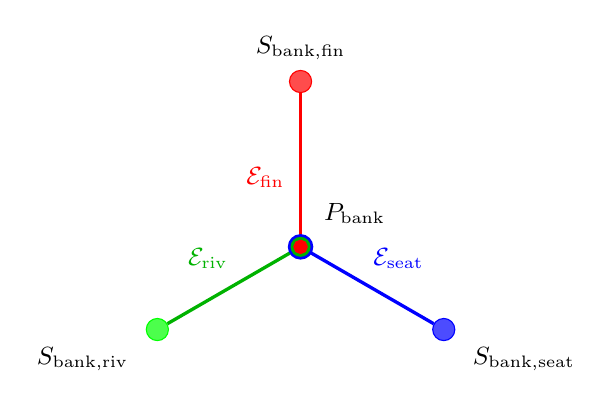
\begin{tikzpicture}[scale=0.5,
    outer/.style={circle, draw, minimum size=8pt,
                  inner sep=0pt, font=\footnotesize},
    lab/.style={font=\small}]
% central shared reference-subspace vertex
\coordinate (c) at (0,0);

\node[lab, above right=7pt] at (c)
{$P_{\rm bank}$};

% outer sense-subspace vertices
\node[outer, red, fill=red!70,
      label={[lab]above:
      $S_{{\rm bank},{\rm fin}}$}]
      (fin) at (90:4.2cm) {};

\node[outer, green, fill=green!70,
      label={[lab, xshift=-4pt]below left:
      $S_{{\rm bank},{\rm riv}}$}]
      (riv) at (210:4.2cm) {};

\node[outer, blue, fill=blue!70,
      label={[lab, xshift=4pt]below right:
      $S_{{\rm bank},{\rm seat}}$}]
      (seat) at (330:4.2cm) {};

% hyperedges labelled by context
\draw[very thick, red] (c) --
      node[lab, left=2pt, pos=0.45]
      {$\mathcal E_{\rm fin}$} (fin);

\draw[very thick, green!70!black] (c) --
      node[lab, above left=1pt, pos=0.45]
      {$\mathcal E_{\rm riv}$} (riv);

\draw[very thick, blue] (c) --
      node[lab, above right=1pt, pos=0.45]
      {$\mathcal E_{\rm seat}$} (seat);

% central concentric disks
\filldraw[blue, very thick] (c) circle (8pt);
\filldraw[green!70!black, very thick] (c) circle (6pt);
\filldraw[red, very thick] (c) circle (4pt);
\end{tikzpicture}
\caption{%
Structural incidence schematic for the lexically ambiguous token ``bank.''
The center is the shared lexical projector $P_{\rm bank}$; outer nodes show
residual sectors for financial, river-edge, and seat/bench contexts.  Each arm
is a fragment of a context hyperedge; omitted orthogonal projectors complete
its basis.  If $m_s>1$, an $S_{t,s}$ node aggregates several rank-one vertices
and is not itself one rank-one outcome.  Concentric colors mark membership of
the same projector in all three contexts.  The diagram records incidence only:
it is neither a causal map nor a Born-rule measurement, and it is not a picture
of the Arora vector sum in Eq.~\eqref{eq:arora-mixture}.
}
\label{fig:reference-subspace}
\end{figure}

Figure~\ref{fig:reference-subspace} illustrates the shared-incidence structure.
Its label $\mathcal E_s$ denotes the completed projector family, or context
hyperedge, for linguistic context class $s$; the drawing shows only the part
that contains the common projector and the indicated residual sector.

\subsection{Classical filters for the optional shared-anchor model}
\label{sec:classical-filters}

Collect the residual basis vectors in
$B_{t,s}=[u_{t,s,1}\ \cdots\ u_{t,s,m_s}]$.  Equation~\eqref{eq:sense-subspace}
says that $B_{t,s}\T B_{t,s}=I$ and $B_{t,s}\T r_t=0$.  Thus
$B_{t,s}B_{t,s}\T$ is the orthogonal projector onto $S_{t,s}$, while
$P_t=r_t r_t\T$ projects onto the fixed lexical ray.

The low-rank classical filter associated with context class $s$ is
%
\begin{equation}
\label{eq:context-projector}
\Pi_{t,s}=P_t+B_{t,s}B_{t,s}\T .
\end{equation}
Because the two bases are orthonormal and perpendicular, their cross products
vanish.  Squaring $\Pi_{t,s}$ therefore returns $\Pi_{t,s}$ itself.  This
idempotence is the defining property of the orthogonal projector onto the
direct sum $\mathcal R_t\oplus S_{t,s}$.
All $\Pi_{t,s}$ preserve the same direction $r_t$ and differ only in the
displayed residual sectors.  They are partial filters, not complete quantum
measurement contexts: further mutually orthogonal directions must be added to
complete the basis described above.  No Born probability is assigned to these
filters.

Their ordinary matrix action is concrete:
%
\begin{equation}
\label{eq:context-filter}
h_{t,s}^{(\Pi)}(x)
=\Pi_{t,s}h(x)
=P_t h(x)+B_{t,s}B_{t,s}\T(I-P_t)h(x).
\end{equation}
%
The first term retains the component along the lexical anchor; the second
retains only the residual component selected by context class $s$.  One may select a
single $s$ or take a context-dependent soft mixture as in
Sec.~\ref{sec:attention}.  Equations~\eqref{eq:context-projector} and
\eqref{eq:context-filter} define a proposed constrained module or probe; they
do not claim that current LLMs already implement it.  Quantum-logic discussions
sometimes call contexts with shared outcomes \emph{intertwining} or
interlocking.  Here that word refers only to the shared hypergraph incidence,
not to an operator equation or physical quantum process.  Everything here uses
ordinary real matrices on classical hardware.

\subsection{Readout in the optional shared-anchor model}
\label{sec:gated}

Let $h(x)\in\R^d$ be a contextual state and retain the orthogonal projector
$P_t$ defined above. The two components are
%
\begin{align}
\label{eq:reference-decomp}
h(x)&=h_{\rm ref}(x)+h_\perp(x),\\
h_{\rm ref}(x)&=P_t h(x),\nonumber\\
h_\perp(x)&=(I-P_t)h(x)\in\mathcal R_t^\perp.\nonumber
\end{align}
%
The orthogonal projection theorem makes this decomposition unique:
$P_th$ is the closest vector in $\mathcal R_t$ to $h$, and $(I-P_t)h$ is
perpendicular to that subspace.  Pythagoras gives
$\norm h^2=\norm{P_th}^2+\norm{(I-P_t)h}^2$.
The hypothesis is that most sense-disambiguating variation is present in
$h_\perp(x)$, not that the decomposition itself is special.  A
basis-invariant score can be expressed directly with the orthonormal matrices
already defined:
%
\begin{align}
\label{eq:sense-coordinates}
e_t(x)&=|r_t\T h(x)|^2=\norm{P_t h(x)}^2,\nonumber\\
\beta_{t,s}(x)&=B_{t,s}\T h_\perp(x),\\
f_{t,s}(x)&=\norm{\beta_{t,s}(x)}^2
=\norm{B_{t,s}B_{t,s}\T h_\perp(x)}^2.\nonumber
\end{align}
%
The scalar $r_t\T h$ and the entries of $B_{t,s}\T h_\perp$ are ordinary
coordinates in orthonormal frames.  Parseval's identity says that the sum of their squared
coordinates equals the squared length of the corresponding orthogonal
projection.  This is why the energies do not depend on the particular
orthonormal basis chosen inside the same subspace.
Here $e_t$ measures energy along the candidate lexical ray and $f_{t,s}$
measures projection energy in the candidate residual subspace.  The latter is
invariant under changes of orthonormal basis within the same residual subspace.
An illustrative projection-energy score is
%
\begin{equation}
\label{eq:sense-score}
\gamma_{t,s}(x)=\frac{f_{t,s}(x)}{m_s}.
\end{equation}
%
The division by the subspace rank matters when the $m_s$ differ: for an
isotropic residual, expected raw projection energy is proportional to rank.
With equal ranks it does not change the ordering.  A more careful empirical
implementation may instead calibrate each raw energy against its own held-out
null distribution.
The selected context-class label is
%
\begin{equation}
\label{eq:selected-sense}
s^*(x)=\argmax_s \gamma_{t,s}(x).
\end{equation}
%
Multiplying every $\gamma_{t,s}$ by the same positive function of $e_t$ would not
change this ranking; reference energy can instead supply an independently
calibrated engagement or abstention threshold.  The score is an illustrative
probe, not a derivation of how an LLM
must disambiguate.  At test time the true sense label is unavailable, so a
practical implementation must learn the router from context without oracle
access.  The empirical content is the proposed separation of roles: the
anchor component tracks token identity or engagement, while the orthogonal
component contains sense-disambiguating information. If no token-associated
$\mathcal R_t$ exposes sense structure better than centered, token-mean,
frequency-controlled, layer-matched, and random controls, the hypothesis
fails.

\subsection{From static mixtures to dynamic contextual embeddings}
\label{sec:dynamic}

Transformers already handle lexical ambiguity dynamically.  Every occurrence
of token type $t$ begins with the same embedding-table row, apart from position
information, but its later hidden state $h_\ell(t\mid x)$ depends on the
surrounding sequence $x$.  Thus the static mixture in
Eq.~\eqref{eq:arora-mixture}, the interpretable reweighting model in
Eq.~\eqref{eq:classical-sense-reweighting}, and an actual Transformer hidden
state are three different objects.  The first describes a corpus-level type
vector, the second is a classical latent-sense model, and only the third is the
output of the network's layers.  The network is not guaranteed to recover the
hypothetical $q_{t,s}$ or to implement their convex mixture literally.

The shared-anchor proposal adds a constraint on the occurrence states; it is
not an alternative hardware architecture and is not needed for ordinary
contextualization.

Its strict form preserves the same token-associated vector $a_t r_t$ at a
chosen representation layer:
%
\begin{align}
\label{eq:layer-decomp}
\widetilde h_\ell(t\mid x)
&=a_t r_t+z_\ell(t,x),\\
r_t\T z_\ell(t,x)&=0 .\nonumber
\end{align}
%
Here $a_t$ is learned for token type $t$ but does not depend on $x$; hence
$a_t r_t$ is literally the same lexical component in every use.  The residual
$z_\ell(t,x)$ depends on the surrounding text and carries the contextual
variation.  For an unconstrained pretrained model, the identity
$h=P_th+(I-P_t)h$ is automatic, but constancy of the coefficient
$r_t\T h_\ell(t\mid x)$ is not.  One can therefore test a weaker diagnostic
version by measuring that coefficient's held-out variation, or enforce the
strict version in a fitted adapter.

The hypothesis predicts that the residual carries useful disambiguating
information and lies near the low-dimensional subspace $S_{t,s}$ selected by the
context.  Labeled senses should be more separable in $\mathcal R_t^\perp$ than
in complements of matched control rays.

Thus the critical question is not whether contextual embeddings move; they
do.  It is whether the same lexical anchor can be retained while their
sense-relevant residual movement is organized by residual subspaces, and whether
that constraint predicts held-out data better than matched untied or
unstructured models.

% ======================================================================
\section{Attention and classical context-dependent reweighting}
\label{sec:attention}
% ======================================================================

A standard attention head computes
%
\begin{equation}
\label{eq:attention}
h'=\sum_j\alpha_j v_j,
\qquad
\alpha_j=
\frac{\exp(q_{\rm att}\T k_{{\rm att},j}/\sqrt{d_{\rm head}})}
{\sum_{j'}\exp(q_{\rm att}\T k_{{\rm att},j'}/\sqrt{d_{\rm head}})} .
\end{equation}
%
$q_{\rm att},k_{{\rm att},j}\in\R^{d_{\rm head}}$ are the query and key
vectors of that head, and $v_j$ is its value vector.  The local head width
$d_{\rm head}$ is an architectural
quantity, not necessarily the selected carrier dimension $d$ used in the
geometric null model.
Keys determine the attention coefficients, while values are the vectors being
averaged.  Because they are produced by different learned maps, ordinary
attention is routing rather than orthogonal projection or basis
reconstruction.

Softmax makes every $\alpha_j$ nonnegative and makes the coefficients sum to
one, so $h'$ is a convex combination of the value vectors.  Cauchy--Schwarz
bounds a raw query--key score by the product of their lengths.  The factor
$1/\sqrt{d_{\rm head}}$ keeps typical score fluctuations of order one when
many roughly independent coordinate contributions are added.
This statement concerns the pre-output aggregate of one head.  A complete
multi-head attention block subsequently applies output maps and a residual
connection, so the block as a whole need not be a convex combination.

Attention can emphasize information carried by some positions more than
others, but the measurement metaphor is unreliable.  In the terminology of
Sec.~\ref{sec:reference}, its output can help a later computation infer which
sense is plausible.  It is not, however, the orthogonal projection used in the
optional geometric model, and there is no general ``collapse'' onto one sense.

A usable context selector cannot receive the true sense label at inference.
Let learned router logits $\ell_{\theta,s}(x,t)$, with router parameters
$\theta$, depend only on the available
sequence and token state, and define
%
\begin{equation}
\label{eq:context-temp}
p_\theta(s\mid x,t)=
\frac{\exp(\ell_{\theta,s}(x,t)/\tau_{\rm r})}
{\sum_{s'}\exp(\ell_{\theta,s'}(x,t)/\tau_{\rm r})},
\qquad \tau_{\rm r}>0 .
\end{equation}
%
Here $\tau_{\rm r}$ is the router temperature: larger values flatten the
context-class probabilities and smaller values sharpen them.  These are ordinary
classical conditional probabilities learned from linguistic data.  They are
not Born probabilities and are not constrained by Gleason's theorem.
If positive corpus sense frequencies are available, one may include the static
prior by multiplying each unnormalized weight by $\pi_t(s)$:
%
\begin{equation}
\label{eq:context-with-prior}
p_\theta^{\rm prior}(s\mid x,t)=
\frac{\pi_t(s)\exp(\ell_{\theta,s}(x,t)/\tau_{\rm r})}
{\sum_{s'}\pi_t(s')\exp(\ell_{\theta,s'}(x,t)/\tau_{\rm r})}.
\end{equation}
%
A uniform prior reduces to Eq.~\eqref{eq:context-temp}.  Equivalently, one can
add $\tau_{\rm r}\log\pi_t(s)$ to the logit before dividing by
$\tau_{\rm r}$.  This is ordinary probabilistic reweighting, not a quantum
amplitude update.
The router may use the illustrative score in Eq.~\eqref{eq:sense-score}, but
need not do so.  To write the strict shared-anchor code explicitly, let
$z_{t,s}(x)\in\R^{m_s}$ be residual coordinates produced from the sequence.
Then
%
\begin{equation}
\label{eq:shared-anchor-code}
h_t^{\rm prop}(x)=a_t r_t+
\sum_s p_\theta(s\mid x,t)B_{t,s}z_{t,s}(x).
\end{equation}
%
Require $a_t\ne0$ and choose a nondegeneracy criterion on training data so that
the anchor carries measurable token information rather than collapsing to a
negligible component.  The first term is independent of $x$; the router weights, residual coordinates,
and therefore the complete representation are context dependent.  Hard routing
keeps only the residual subspace with the largest probability.  A diagnostic that filters
an already observed hidden state instead uses
%
\begin{equation}
\label{eq:soft-context-filter}
\bar h_t(x)=\sum_s p_\theta(s\mid x,t)\,\Pi_{t,s}h(x).
\end{equation}
%
The effective operator
$\sum_s p_\theta(s\mid x,t)\Pi_{t,s}$ is generally not idempotent and hence is
not itself an orthogonal projector.  Squaring a weighted sum creates cross
terms, so the result need not equal the original sum.  Attention may supply its routing signal,
but neither the shared anchor nor the subspace structure follows from standard
attention.  The constrained model must therefore be compared with
parameter-matched mixture-of-experts and unstructured low-rank alternatives.

For an implementable adapter at a chosen layer, let
$Z_{t,s}\in\R^{d\times m_s}$ be a trainable seed matrix such that
$(I-P_t)Z_{t,s}$ has full column rank, and set
$B_{t,s}=\operatorname{orth}((I-P_t)Z_{t,s})$, where
$\operatorname{orth}$ means ordinary Gram--Schmidt orthonormalization or an
equivalent matrix factorization.
Multiplication by $I-P_t$ first removes every component along the shared ray;
full column rank ensures that $m_s$ independent residual directions remain.
Tie the same $r_t$ across all $s$, compute the router, and obtain $\bar h_t$
from Eq.~\eqref{eq:soft-context-filter}.  The filtered state may be used as a
diagnostic probe.  A strict shared-anchor adapter instead forms the
post-adapter state
%
\begin{equation}
\label{eq:strict-anchor-update}
h_t^+(x)=a_t r_t+(I-P_t)\bigl[h(x)+\lambda_{\rm gate}U\bar h_t(x)\bigr],
\end{equation}
%
where $U\in\R^{d\times d}$ is a learned output map and $\lambda_{\rm gate}$ is
a scalar gate.
Multiplication by $I-P_t$ ensures $P_t h_t^+(x)=a_t r_t$ for every $x$; in plain
language, it keeps the learned residual update perpendicular to the fixed
anchor.  The router, residual subspaces, residual-coordinate maps, and adapter are then
trained on a language-model or task loss.  Held-out evaluation must compare
against adapters with the same ranks and parameter count but no shared-anchor
constraint.

% ======================================================================
\section{Discussion}
\label{sec:discussion}
% ======================================================================

The chapter's positive geometric thesis is the abundance--access distinction.
At a fixed angular tolerance, high dimension permits an exponentially large
finite dictionary, but a decoder still pays for the features that activate
together.  The corresponding semantic hypothesis is concrete: training should
allocate lower task-weighted cross-talk to important, frequently coactive
features than appears in isotropic and activity-matched controls.

For lexical ambiguity, the classical starting point is a static
frequency-weighted sense mixture, followed by context-dependent occurrence
states.  The shared-anchor residual-subspace proposal adds a separate and
strictly stronger inductive bias.  Reusing one lexical ray across context
classes may reduce sample complexity when the common component is real and
per-use data are scarce.  It does not add expressive power, and it should lose
when forced sharing is wrong.  Learning curves against the simpler mixture,
ordinary contextual models, and equally expressive unstructured adapters
therefore test the proposed mechanism directly.

\subsection{Relation to neural feature superposition and sparse autoencoders}
\label{sec:superposition}

Neural feature superposition is the second item in
Sec.~\ref{sec:five-superpositions}.  It proposes that a layer state can contain
more candidate features than independent coordinates by using a sparse linear
combination of generally nonorthogonal directions
\cite{elhage2022superposition,bricken2023monosemanticity}.  In
Eq.~\eqref{eq:hidden}, the feature amplitudes $x_j$ may be signed, need not add
to one, and are not sense probabilities.  This differs both from the convex
lexical mixture in Eq.~\eqref{eq:arora-mixture} and from a quantum state.

The null model separates dictionary coexistence from simultaneous linear
readout.  In the isotropic, weak-dependence model, many directions can coexist
while a fixed-target correlation decoder accumulates interference of scale
$\sqrt{k/d}$.  Sparse activity reduces the number of simultaneous cross terms
for this decoder; it is not asserted to be universally necessary for
structured dictionaries or nonlinear recovery.  Nor does Arora et al.'s
sparse lexical factorization establish that its learned atoms obey the
quasi-orthogonality condition of Eq.~\eqref{eq:quasiortho}.

Sparse autoencoders (SAEs) give a concrete empirical interface. They
approximate layer activations as sparse expansions over learned decoder
directions, making the $w_i$ of Eq.~\eqref{eq:hidden} measurable
objects rather than hypothetical features. Recent work has scaled SAEs,
studied SAE feature geometry, and automated interpretation of large
numbers of latents~\cite{gao2025scaling,li2025geometry,paulo2025automatically,shu2025survey}. In the
present framework, SAE decoder directions make the L\'evy/JL calibration and
coactivation-weighted diagnostic measurable, while sense-conditioned SAE
activation clusters can test the stronger shared-anchor residual-subspace hypothesis.

\subsection{Why the lexical mixture is not a full quantum superposition}

There is no algebraic obstacle to taking a full \emph{classical} linear sum of
sense vectors: Eq.~\eqref{eq:arora-mixture} already does so.  What cannot be
added merely by changing terminology is quantum coherence.  In an orthonormal
quantum basis $\{\lvert s\rangle\}$, a normalized pure state has the form
%
\begin{equation}
\label{eq:quantum-coherent-state}
\lvert\psi\rangle=\sum_s c_s\lvert s\rangle,
\qquad c_s=\sqrt{p_s}e^{i\phi_s},
\qquad \sum_s|c_s|^2=1 .
\end{equation}
%
The phases $\phi_s$ are operational only if a later measurement can recombine
the alternatives and reveal interference.  An incoherent quantum mixture is
instead represented by a density matrix
%
\begin{equation}
\label{eq:quantum-mixture}
\rho_{\rm mix}=\sum_s p_s\lvert s\rangle\langle s\rvert .
\end{equation}
%
Here $p_s\geq0$ and $\sum_s p_s=1$.  A density matrix is a positive
semidefinite matrix of trace one, and
$\lvert s\rangle\langle s\rvert$ is the rank-one projector onto basis
direction $s$.  By contrast, the pure-state density matrix contains
%
\begin{equation}
\label{eq:pure-density-coherences}
\lvert\psi\rangle\langle\psi\rvert
=\sum_{s,t}c_sc_t^*\lvert s\rangle\langle t\rvert .
\end{equation}
%
The star means complex conjugation.  Terms with $s\ne t$ are the off-diagonal
coherences; they are absent from $\rho_{\rm mix}$ in this basis.
The Arora vector $\sum_s\pi_t(s)q_{t,s}$ is neither object: it is a barycenter
of real lexical vectors, not a state amplitude and not a density operator.
Ordinary Euclidean cross terms do not by themselves demonstrate quantum
interference.

A genuinely quantum-style lexical model would therefore need more than the
word \emph{superposition}.  It would have to specify an orthonormal outcome
space, quantum amplitudes (real or complex), any relative phases, which
linguistic operations act as measurements, and an empirical probability law showing phase-sensitive
interference.  The present chapter supplies none of these, and ordinary
self-attention supplies no Born rule.  Introducing the full apparatus without
such evidence would add parameters and nonidentifiability rather than explain
polysemy.

\subsection{Relation to quantum cognition and compositional semantics}
\label{sec:related-quantum}

The phrase ``quantum-inspired'' has an established cognitive and linguistic
lineage.  Quantum-cognition models use Hilbert-space states, projectors,
interference, and order effects as mathematical models of human judgment and
concept combination, without requiring quantum processes in the brain
\cite{Busemeyer2012,aerts2005b}.  Work on the human mental lexicon has likewise
used quantum structure to model word-association and memory experiments
\cite{bruza2009lexicon}.  Those studies concern behavioral probabilities and
conceptual judgments; the present chapter concerns hidden representations and
learned readout in an LLM.

A different but neighboring tradition is compositional distributional
semantics.  Coecke, Sadrzadeh, and Clark combine vector-space word meanings
with grammatical composition through tensor and categorical maps
\cite{coecke2010compositional}.  That construction shows how tensor products
can organize composition, but it does not establish that a Transformer
residual stream has a fully accessible semantic tensor factorization
$d=q^n$.

The optional shared-anchor model is a classical tied-subspace adapter: a router
mixes context-conditioned residual subspaces that share one lexical ray.  Its
quantum-logic inspiration is exhausted by that incidence fact.  It does not
invoke noncommuting observables, order effects, complex amplitudes, unitary
dynamics, or Born probabilities.  Calling it quantum-inspired identifies the
source of one structural constraint, not the physical nature of the
computation and not a general account of polysemy.

\subsection{Limitations}
\label{sec:limitations}

The limitations can be grouped into five issues.

\emph{Geometry.}  L\'evy's lemma controls a fixed Lipschitz probe; a finite
dictionary additionally needs a union bound or code construction.  JL gives
an existence scale, the random-code formula gives an ensemble calibration,
and the Welch bound gives a deterministic floor.  None is a semantic upper
bound.

\emph{Measurement protocol.}  The usable rank $d$ and dictionary size $\Msem$
depend on layer choice, whitening, feature extraction, normalization, and
duplicate removal.  Contextual states can be anisotropic
\cite{ethayarajh2019,gao2019representation,mu2018allbutthetop,razzhigaev2024shape},
although anisotropy is not universal~\cite{machina2024anisotropy}.  Whitening
changes the inner product and therefore changes angles.  Finite-dimensional
norm equivalence preserves convergence and continuity, but it does not
preserve numerical angles or coherence.  Every comparison must therefore use
one declared metric and selection rule.

\emph{Readout.}  The law $\sint\sim\sqrt{k/d}$ concerns one correlation
decoder under random-like cancellation.  Structured dictionaries, nonlinear
decoders, inactive-feature comparisons, and correlated errors can change it.
Likewise, Eq.~\eqref{eq:int-energy} omits cross-moment terms unless the stated
zero-cross-moment assumption holds.

\emph{Polysemy models.}  Equation~\eqref{eq:arora-mixture} is conditional on a
generative model and an asymptotic training argument.  A single vector has no
unique decomposition into senses; sparse recovery adds assumptions and shared
corpus structure.  Discourse atoms need not be individual senses, and Arora
et al. do not establish their global quasi-orthogonality.  For a modern
Transformer, neither the input table nor an intermediate hidden state is
guaranteed to obey the same mixture law.  Attention can transform and route
information without being a projector onto a sense.

\emph{Shared-anchor residual-subspace model.}  The model may simply be wrong.  Token identity
can make its weak version pass while its nontrivial held-out comparison fails.
Anchors, ranks, residual subspaces, and routers must be fixed on training data, and the true
sense label is unavailable at test time.  The proposed controls decide whether
the tied model adds held-out value beyond ordinary token identity, clustering,
and equally expressive untied adapters.

\subsection{Proposed experiments and failure criteria}
\label{sec:predictions}

No experiment is reported in this chapter.  The purpose of this section is to
turn the analytical claims into a staged, falsifiable program.  The first
stage calibrates geometry; the later stages test increasingly restrictive
semantic structure.

\emph{Geometric calibration (not a semantic claim).}
For a dictionary independently established to be overcomplete, compare its
coherence, overlap distribution, and fixed-target readout error with isotropic
and activity-matched controls.  Agreement with Eq.~\eqref{eq:max-overlap} is a
baseline result, not evidence that overcompleteness is useful; departure from
it must be diagnosed before being called learned structure.  JL itself is a
theorem; the empirical question is whether task-relevant geometry and readout
survive projection near its logarithmic dimension scale.

\emph{Claim M0: static-mixture baseline.}
Sense-labelled embeddings or independently estimated sense centroids, obtained
in the same lexical carrier or mapped into it using training data only,
reconstruct a held-out static type vector by the frequency-weighted rule in
Eq.~\eqref{eq:arora-mixture} better than shuffled or frequency-matched
components.  This tests the model-dependent classical precursor, not quantum
coherence and not the shared anchor.

\emph{Claim M1: contextual reweighting.}
Weights inferred from the surrounding text improve held-out sense prediction
or reconstruction over the corpus prior $\pi_t(s)$, static sparse coding, and
ordinary clustering.  A positive result supports a classical contextual
mixture; it does not show that the Transformer's internal computation is
literally that mixture.

\emph{Claim A0: token-component sanity check.}
A token-associated component explains cross-context variation shared by
occurrences of the same token and carries nonnegligible held-out token
information relative to matched random rays.  This weak result is expected and
is not evidence for a privileged semantic sector, but it prevents the strict
model from passing with a zero or negligible anchor.

\emph{Claim A1: nontrivial shared-anchor claim.}
Relative to token-mean subtraction, top-principal-component removal, and
same-rank random or supervised controls, a nondegenerate lexical ray
$\mathcal R_t$ fixed from training data exposes held-out predictive information
in $\mathcal R_t^\perp$ while its anchor coefficient remains sufficiently
stable across contexts for a normalized tolerance fixed on training data.  A0
is a prerequisite for A1.

\emph{Claim B: low-dimensional residual subspaces.}
Within $\mathcal R_t^\perp$, context-conditioned residuals admit a cross-validated
low-rank description that predicts or compresses held-out states better than
shuffled-label, ordinary clustering, and matched-subspace controls.  Related
polysemous senses need not have minimal cross-sense coherence.

\emph{Claim C: useful shared-anchor context classes.}
Without access to the true sense label at inference, a router and residual
subspaces tied through the same lexical anchor improve held-out prediction,
compression, interpretability, or sample efficiency relative to
parameter-matched untied subspaces, unstructured low-rank adapters, and
mixture-of-experts controls.  The predicted advantage is largest for scarce or
imbalanced senses and may vanish when no stable shared component exists.

These claims can fail independently.  The geometric calibration can hold while
all lexical claims fail.  M0 can hold while M1 fails, or both can hold while
every shared-anchor claim fails.  A0 may pass while A1 fails; that outcome
would reject a privileged lexical anchor without denying ordinary token
identity.  Claim B can hold relative to a non-token-associated subspace, and
A1 and B can hold even if the tying in Claim C adds no predictive value.

\paragraph{Minimum pilot.}
A small first study needs no retraining of the language model.  Choose one
public model, one
layer, and a prespecified sample of ambiguous tokens from SemCor or the
Word-in-Context (WiC) benchmark~\cite{pilehvar2019wic}.  Estimate candidate token
means and top principal components on the training split only.  SemCor supports
a linear sense classifier; for WiC use its intended pairwise same-sense versus
different-sense task.  Compare full states, residuals after each candidate
removal, and same-rank random controls.  Also report held-out anchor energy,
token-identification information, and normalized coefficient variation.
Together, held-out accuracy, calibration, nondegeneracy, and stability decide
A1.
Adding sparse-autoencoder features then tests the coactivation statistic.  A
failure at this stage should stop the tied-subspace study rather than be
hidden by a more flexible router.

The following tests separate the possibilities.

\begin{enumerate}
\item \emph{L\'evy/random-code calibration.}
Fix the carrier metric, spectral threshold or whitening rule, feature extractor,
and duplicate criterion before evaluation.  Report the selected rank $d$,
dictionary size $\Msem$, maximum coherence, the full overlap distribution, and
active-set statistics.  Compare with the Welch floor, isotropic dictionaries,
and controls matched for marginal activity and coactivation.  Treat
Eq.~\eqref{eq:max-overlap} as a finite-sample null prediction, not a pass/fail
capacity test.  Also compare the signed pairwise distribution with the
independently isotropic variance $1/d$; deviations may reflect dependence,
anisotropy, extraction choices, or learned alignment.

\item \emph{JL projection-stability test.}
Fix a finite evaluation set of $\Msem$ normalized directions or contextual
states, include the origin, and prespecify a relative squared-distance
distortion $\delta_{\rm JL}$.  Project to $d_{\rm proj}$ dimensions using
frozen random maps scaled to preserve squared lengths on average, and measure
pairwise distortion and held-out task
performance as $d_{\rm proj}$ varies.  JL predicts metric preservation when
$d_{\rm proj}$ is proportional to
$\delta_{\rm JL}^{-2}\log(\Msem+1)$ up to universal constants; preservation of
semantic performance is the additional empirical question.  Compare random
Gaussian or orthogonal maps with learned low-rank maps at the same
$d_{\rm proj}$.

\item \emph{Classical polysemy baselines.}
For static embeddings, estimate sense vectors without using the held-out type
vector, then compare frequency-weighted reconstruction with shuffled senses
and matched random components.  In a separate sparse-dictionary baseline,
learn discourse atoms and their sparse coefficients rather than assigning
corpus sense frequencies to atoms.  Then compare the contextual weights in
Eq.~\eqref{eq:classical-sense-reweighting} with a
prior-only mixture, ordinary contextual probes, clustering, and an unconstrained
router.  Report reconstruction and sense-prediction performance before imposing
any shared ray.  These baselines decide M0 and M1 and prevent the optional
incidence model from receiving credit for ordinary contextualization.

\item \emph{Shared-anchor test.}
For a lexically ambiguous token, choose candidate lexical rays generated
by the mean contextual embedding, a static input embedding explicitly mapped
into the same layer carrier,
or a learned token-specific direction.  Fix the candidate on training data,
then project held-out layer states with $P_t$ and $I-P_t$ as in
Eq.~\eqref{eq:reference-decomp}.  Report the variation of the anchor coefficient
$r_t\T h_\ell(t\mid x)$ across contexts; exact constancy is the strict model,
while any relaxed tolerance must be chosen before seeing test results.  Sense labels
should be better separated in $\mathcal R_t^\perp$ than in orthogonal
complements of random, frequency-matched, or layer-matched control rays, and
than in separately centered, token-mean-subtracted, or
top-principal-component-removed baselines.  Require the candidate anchor to
carry prespecified nonnegligible token energy or token-identification
information relative to matched random rays; report a normalized stability
statistic such as
$\Var_x(r_t\T h_\ell(t\mid x))/\E_x\norm{h_\ell(t\mid x)}^2$,
where $\Var_x$ and $\E_x$ are the empirical variance and mean over held-out
occurrences of the token.
Compare held-out classification, compression, or a prespecified measure of
added predictive information, with uncertainty estimated by label shuffling
and resampling token instances.

\item \emph{Operational residual-subspace test.}
For each sense $s$, collect projected states
$z_\ell(t,x)\in\mathcal R_t^\perp$ and estimate a low-rank subspace by
principal component analysis (PCA) or probabilistic factor analysis.  PCA is
an application of the spectral theorem to the sample covariance matrix: its
directions are eigenvectors with the largest eigenvalues.  Select $m_s$
without test-label leakage and use
an orthonormal basis $B_{t,s}$.  Evaluate held-out reconstruction and sense
prediction against shuffled labels, ordinary supervised subspaces, and
unsupervised clustering of equal rank.  Report
$\opnorm{B_{t,s}\T B_{t,s'}}$ descriptively, without assuming related senses
must be nearly orthogonal.

\item \emph{Anchor-versus-residual readout test.}
For the relaxed diagnostic states, rather than the strict fitted model in
Eq.~\eqref{eq:strict-anchor-update}, linear probes trained on
$z_\ell(t,x)$ should perform comparably to
probes trained on the full state $h_\ell(t\mid x)$, while probes
restricted to the anchor component $P_t h_\ell(t\mid x)$ should provide
less incremental sense information after frequency, syntax, and sense-prior
controls.  Near-chance performance is not required because the reference
component may legitimately retain correlated information.

\item \emph{Shared-anchor residual-subspace test.}
Fit $r_t$, $B_{t,s}$, the residual-coordinate maps, and the router on training
sequences, then evaluate Eqs.~\eqref{eq:shared-anchor-code} and
\eqref{eq:soft-context-filter} without true sense labels on held-out instances.
Compare with untied subspaces, unstructured low-rank adapters, ordinary contextual
probes, parameter-matched mixture-of-experts models, and shuffled subspace or
sense labels.
Repeat the comparison across training-set sizes and sense-imbalance levels.
The tying mechanism predicts a larger advantage in the low-data regime and no
guaranteed advantage when data are abundant or the shared component is weak.

\item \emph{Synthetic concurrency degradation.}
At a fixed layer, inject controlled classical feature sums
%
\begin{equation}
h_k=h_0+\lambda\sum_{j=1}^k x_j w_j,
\end{equation}
%
where $h_0$ is a held-out baseline activation, the $w_j$ are independently
chosen unit injection directions, the coefficients $x_j$ are independent,
centered, and unit-variance, and $\lambda$ controls injection amplitude.  The
directions may come, for example, from SAE decoder directions or frozen linear
probes.  For random-like directions under the specified correlation decoder,
the injected fixed-target interference has RMS scale
$\lambda\sqrt{k/d}$, up to the distinction between $k$ and $k-1$.
How that interference changes downstream task performance is an empirical
question.  Include norm-preserving, random-direction, activation-frequency,
and out-of-distribution controls; degradation by itself does not validate a
semantic or quantum interpretation.

\item \emph{Coactivation-dependent geometry.}
At matched marginal activation frequency, feature similarity, SAE
reconstruction error, amplitude, and task relevance, important frequently
coactive features should contribute less to Eq.~\eqref{eq:int-energy} than
activity-matched controls.  This tests learned redistribution of interference,
independently of the shared-anchor hypothesis.
\end{enumerate}

\subsection{Scope of the optional quantum-incidence analogy}
\label{sec:quantum}

The optional shared-anchor implementation is classical: a router mixes real
low-rank residual subspaces tied through one real lexical ray.  Its
quantum-logic inspiration consists of one structural fact.  A maximal
projective measurement context can be represented by mutually orthogonal
rank-one projectors whose sum is the identity matrix.  In dimension at least
three, distinct contexts can contain the same projector $P_t$ while differing
in their other members.  Figure~\ref{fig:reference-subspace} copies only that
shared-incidence pattern.  Incidence is not addition: the picture neither
represents the sum in Eq.~\eqref{eq:arora-mixture} nor follows merely because
two linguistic senses reuse some features.

The analogy does not itself encode polysemy.  If the prepared quantum state
were exactly the shared pure state $P_t$, the Born rule would give
$\operatorname{tr}(P_tP_t)=1$ in every context containing it; the result would
be deterministic.  More generally, for a fixed state $\rho$, the probability
$\operatorname{tr}(\rho P_t)$ of the same shared outcome does not depend on
which compatible projectors complete the basis.  Gleason's theorem, under its
additivity assumptions in dimension at least three, characterizes such
projector probabilities by a density matrix~\cite{Gleason,ramanathan-2024}.
In the language model, by contrast, router weights, residual coordinates, and
the complete occurrence representation depend deliberately on linguistic
context $x$.  The router is learned by ordinary optimization and obeys no Born
or Gleason rule.

Thus the comparison is partly negative.  Arora's mixture is ordinary vector
addition; Transformer contextualization is an ordinary learned map; and the
optional tied adapter borrows only a hypergraph incidence pattern.
Noncommuting matrices, order effects, complex phases, unitary dynamics, and
physical quantum states are not part of the proposal.

This limited probability consistency should not be paraphrased as saying that
quantum mechanics is wholly noncontextual.  Kochen--Specker results concern the
impossibility of certain global noncontextual sharp-value assignments
\cite{specker-60,kochen1}; no analogous theorem is claimed for semantic
embeddings.  The words ``quantum-inspired'' identify only the source of the
optional shared-incidence constraint, not a quantum explanation of lexical
ambiguity.

% ======================================================================
\section{Conclusion}
\label{sec:conclusion}
% ======================================================================

The central organizing distinction is between abundance and access.
L\'evy concentration,
the Johnson--Lindenstrauss lemma, and random spherical coding are related
expressions of the same high-dimensional concentration phenomenon: at fixed
angular tolerance, a $d$-dimensional carrier admits exponentially many
directions.  The Welch bound gives a deterministic floor on their worst
overlap.  None of these counts makes the directions simultaneously readable.
A simple readout from $k$ random-like active features instead pays an RMS
interference cost of order $\sqrt{k/d}$.

This distinction yields the chapter's positive semantic prediction.  A useful
learned dictionary should not merely contain many directions; it should place
lower task-weighted cross-talk between important features that often
coactivate.  Equation~\eqref{eq:int-energy} turns that idea into a held-out
comparison against isotropic and activity-matched controls.

For lexical ambiguity, the most defensible picture is classical and layered.
A static type vector may approximate a corpus-frequency convex mixture of
sense vectors; surrounding text then produces or helps decode a
context-dependent occurrence state.  Neural feature superposition is a third
classical notion, with sparse and generally nonprobabilistic feature
coefficients.  None is a quantum-coherent superposition, and ordinary
attention is not a measurement-induced collapse.

The tied shared-anchor adapter is retained only as an optional stronger
hypothesis.  It preserves a fixed lexical component while surrounding text
selects or mixes low-rank residual context subspaces.  Sharing may improve
sample efficiency when a genuine common component exists and per-sense data
are scarce, but the minimum pilot in Sec.~\ref{sec:predictions} can reject it.
Its sole quantum-logic-inspired element is the incidence pattern of one shared
projector in several orthonormal contexts.  That pattern is neither vector
superposition nor an explanation of polysemy; no Born-rule,
noncommutativity, or semantic Kochen--Specker claim is made.
The doubly exponential tensor-product count remains only the conditional
remark of Sec.~\ref{sec:quasiortho}, not a conclusion about ordinary LLMs.

\appendix

% ======================================================================
\section{Explicit formalization of the three computational loops}
\label{app:llm-loops}
% ======================================================================

The following subsections correspond one-to-one to
Secs.~\ref{sec:prose-training}--\ref{sec:prose-online}.  The purpose is not to
specify every engineering detail of a modern model.  It is to identify, in the
order in which they occur, which objects are discrete symbols, which are
vectors, which are temporary results of a calculation, and which are persistent
model parameters.  No argument about the semantic geometry in the main text
depends on this appendix.

We first fix the objects used throughout.  Let $\mathcal S$ be the set of
finite character strings and let $\mathcal V=\{1,\ldots,V\}$ be a finite
vocabulary of $V$ token identifiers.  A token identifier is an integer label;
it is not itself a vector.  For a nonnegative integer $T$, the Cartesian power
$\mathcal V^T$ is the set of token sequences of length $T$; the union below
allows every finite length.  The tokenizer is a fixed, variable-length map
\begin{equation}
\label{eq:app-tokenizer}
\mathsf{Tok}:\mathcal S\longrightarrow
\bigcup_{T\geq0}\mathcal V^T.
\end{equation}
Thus $\mathsf{Tok}$ turns one string into a finite sequence of identifiers.  Its
companion $\mathsf{Detok}$ assembles a token sequence into text.  Apart from any
declared normalization of spaces or characters, detokenization reverses the
tokenization of an admissible string.  Neither map learns a contextual meaning
during the Transformer calculation.

The symbol $d_{\rm model}$ denotes the architectural width of the residual
stream, so every hidden state below is an ordinary real column vector in
$\R^{d_{\rm model}}$.  It must not be confused with the usable semantic carrier
rank $d$ in the main text: restriction, whitening, or removal of inactive
directions may give $d\leq d_{\rm model}$, with equality when the full residual
stream is used.  The symbol $L$ denotes the number of Transformer layers.  The
symbol $\Theta$ denotes the complete
collection of persistent numerical parameters: the token embedding table, the
matrices in all attention and feed-forward blocks, normalization parameters,
and the final vocabulary readout.  If all their entries are written in one long
list, then $\Theta$ may be regarded as a vector in $\R^{N_{\rm par}}$, where
$N_{\rm par}$ is the number of trainable scalar parameters.  This flattening is
only bookkeeping; an implementation stores the parameters as many arrays of
different shapes.  Thus $d_{\rm model}$, $V$, and $N_{\rm par}$ count three
different things: architectural hidden coordinates, token types, and scalar
model parameters.

Persistent parameters survive from one prompt to the next.  Hidden states,
query, key, and value vectors, attention coefficients, and next-token
probabilities are transient quantities recomputed for a particular input.  The
phrase ``attention weight'' is therefore potentially confusing: an attention
coefficient is a temporary number, whereas a model weight is an entry of a
persistent matrix in $\Theta$.  A superscript in parentheses denotes a stage
or index rather than exponentiation: $h_i^{(\ell)}$ will index a layer, while
$\Theta^{(r)}$ with $r=0,1,2,\ldots$ will index a successive parameter update.

\subsection{Creating the weights}
\label{app:training}

This subsection follows Sec.~\ref{sec:prose-training}: text is tokenized,
tokens are represented by vectors, self-attention makes those vectors
context-dependent, a next-token error is calculated, and an optimizer changes
the persistent parameters.

\paragraph{Step 1: turn text into discrete identifiers.}
Consider one training string $\sigma\in\mathcal S$ whose selected training
segment contains $T\geq2$ tokens, so that it supplies at least one next-token
prediction.  Systems often use declared beginning- or end-of-sequence tokens
at document boundaries.  For $i\in\{1,\ldots,T\}$, let
$x_i\in\mathcal V$ denote the identifier at position $i$.  Tokenization gives
\begin{equation}
\label{eq:app-forward-map}
(x_1,\ldots,x_T)=\mathsf{Tok}(\sigma)
\in\mathcal V^T.
\end{equation}
The same identifier may occur several times.  At this stage all
of its occurrences carry the same discrete label, irrespective of context.

\paragraph{Step 2: look up an initial vector and mark its position.}
Let $E_{\rm tok}\in\R^{V\times d_{\rm model}}$ be the token embedding table.  It is one of
the trainable arrays contained in $\Theta$.  Its row
$E_{\rm tok}[a]\in\R^{d_{\rm model}}$ is the lookup vector for token type
$a\in\mathcal V$; square brackets mean table lookup.  In the simplest additive
description, let $\rho_i^{\rm pos}\in\R^{d_{\rm model}}$ be a position vector.
The initial hidden vector $h_i^{(0)}\in\R^{d_{\rm model}}$ is
\begin{equation}
\label{eq:app-initial-state}
h_i^{(0)}=E_{\rm tok}[x_i]+\rho_i^{\rm pos},
\qquad i=1,\ldots,T.
\end{equation}
The superscript $(0)$ means ``before the first Transformer layer.''  The
position vector may be fixed or learned; when it is learned, its entries also
belong to $\Theta$.  Systems using rotary or other positional schemes do not literally add
$\rho_i^{\rm pos}$, but they
serve the same present purpose: the calculation must know both which token
occurred and where it occurred.  Two occurrences of ``bank'' begin with the
same row of $E_{\rm tok}$, but their later hidden states can differ because
their surrounding tokens and positions differ.

\paragraph{Step 3: make the vectors context dependent by self-attention.}
We spell out one attention head in one layer.  Let
$h_i^{(\ell-1)}\in\R^{d_{\rm model}}$ be the vector at position $i$ entering layer
$\ell\in\{1,\ldots,L\}$.  Let $d_{\rm head}$ be the width of one head, and let
$W_Q^{(\ell)},W_K^{(\ell)},W_V^{(\ell)}\in
\R^{d_{\rm head}\times d_{\rm model}}$ be three learned matrices contained in
$\Theta$.  For target position $i$ and source position $j$, write
$q_i,k_j,v_j$ for the three outputs
\begin{equation}
\label{eq:app-qkv}
\begin{aligned}
q_i&=W_Q^{(\ell)}h_i^{(\ell-1)},\\
k_j&=W_K^{(\ell)}h_j^{(\ell-1)},\\
v_j&=W_V^{(\ell)}h_j^{(\ell-1)}.
\end{aligned}
\end{equation}
The vectors $q_i,k_j,v_j\in\R^{d_{\rm head}}$ are called the query, key, and
value.  A query describes what information position $i$ is seeking, a key
describes how position $j$ may be matched, and a value contains the information
to be combined if that position receives attention.  These phrases interpret
three ordinary matrix--vector products; they do not introduce new kinds of
mathematical objects.

For a decoder-only model, position $i$ may attend only to positions
$j\leq i$.  Let $s_{ij}$ denote the real comparison score, let
$\alpha_{ij}$ denote the normalized attention coefficient, and let
$o_i^{\rm att}$ denote the output of this head.  The letter $t$ below is only a
dummy source-position index.  These quantities are
\begin{equation}
\label{eq:app-attention-expanded}
\begin{aligned}
s_{ij}&=\frac{q_i\T k_j}{\sqrt{d_{\rm head}}},\\
\alpha_{ij}
&=\frac{\exp(s_{ij})}
{\sum_{t=1}^{i}\exp(s_{it})},\\
o_i^{\rm att}&=\sum_{j=1}^{i}\alpha_{ij}v_j.
\end{aligned}
\end{equation}
The first line uses the Euclidean inner product.  By the Cauchy--Schwarz
inequality, $|q_i\T k_j|\leq\norm{q_i}\norm{k_j}$, so a large comparison
requires suitably aligned query and key vectors as well as suitable lengths.
The factor $1/\sqrt{d_{\rm head}}$ controls the numerical scale of the scores.
The ordinary exponential function is positive, hence every
$\alpha_{ij}\geq0$, and direct summation gives
$\sum_{j=1}^{i}\alpha_{ij}=1$.  Consequently $o_i^{\rm att}$, the output of
this attention head, is a weighted average, or convex combination, of the
permitted value vectors.  The restriction $j\leq i$
is the causal mask: it prevents the calculation at position $i$ from using the
future target $x_{i+1}$.

A practical layer has several heads.  Their outputs are concatenated, mapped
back to $\R^{d_{\rm model}}$, combined with a residual connection, normalized,
and passed through a feed-forward block.  Denote the resulting vector by
$h_i^{(\ell)}\in\R^{d_{\rm model}}$.  Repeating the procedure for
$\ell=1,\ldots,L$ yields final contextual vectors $h_i^{(L)}$.  Let $F_\Theta$
denote the complete layered Transformer map.  Then
\begin{equation}
\label{eq:app-transformer-map}
(h_1^{(L)},\ldots,h_T^{(L)})
=F_\Theta(h_1^{(0)},\ldots,h_T^{(0)})
\end{equation}
Equation~\eqref{eq:app-transformer-map} collects all these operations into one
function.  During this forward pass
$\Theta$ is fixed.  In contrast, $q_i,k_j,v_j,\alpha_{ij}$, and
$h_i^{(\ell)}$ depend on the current string and are transient.

\paragraph{Step 4: turn the final vector into a next-token distribution.}
Let $W_{\rm out}\in\R^{V\times d_{\rm model}}$ and $b\in\R^V$ be the
vocabulary readout matrix and bias; both belong to $\Theta$.  At training
position $i$, let $g_i\in\R^V$ denote the score vector.  For a candidate token
$a\in\mathcal V$, let $p_\Theta(a\mid x_1,\ldots,x_i)$ denote its predicted
probability given the prefix.  The letter $c$ below is only a dummy token index
in the denominator.  Define
\begin{equation}
\label{eq:app-training-softmax}
\begin{aligned}
g_i&=W_{\rm out}h_i^{(L)}+b,\\
p_\Theta(a\mid x_1,\ldots,x_i)
&=\frac{\exp(g_{i,a})}
{\sum_{c\in\mathcal V}\exp(g_{i,c})}.
\end{aligned}
\end{equation}
The entry $g_{i,a}$ is a real-valued score, often called a logit, not a
probability.  The denominator is a finite sum of positive numbers, so the
softmax expression is nonnegative and
sums to one over $a\in\mathcal V$.  The vertical bar means ``given the prefix
$(x_1,\ldots,x_i)$.''  Because of the causal mask, this distribution depends on
that prefix and not on the unseen suffix $(x_{i+1},\ldots,x_T)$.

\paragraph{Step 5: compare the prediction with the observed continuation.}
Let $P_\Theta(x_2,\ldots,x_T\mid x_1)$ denote the sequence-level conditional
probability assigned to the observed continuation.  The multiplication rule for
conditional probabilities gives
\begin{equation}
\label{eq:app-sequence-probability}
P_\Theta(x_2,\ldots,x_T\mid x_1)
=\prod_{i=1}^{T-1}
p_\Theta(x_{i+1}\mid x_1,\ldots,x_i).
\end{equation}
This product does not assume that tokens are independent: every factor is
conditioned on the entire available prefix.  Taking the negative natural
logarithm turns the product into a sum.  The loss for this string is
\begin{equation}
\label{eq:app-string-loss}
\mathcal L_\sigma(\Theta)
=-\sum_{i=1}^{T-1}
\log p_\Theta(x_{i+1}\mid x_1,\ldots,x_i).
\end{equation}
Each summand is small when the observed next token was assigned a probability
near one and large when it was assigned a probability near zero.

\paragraph{Optional calculus detail: the initial error signal.}
The following derivative may be skipped without losing the computational
sequence.  Let
$\ell_i$ be the $i$th summand in Eq.~\eqref{eq:app-string-loss}, and let the
indicator $\mathbf 1_{\{a=x_{i+1}\}}$ equal one when $a$ is the observed next
token and zero otherwise.  Differentiating the logarithm and softmax gives
\begin{equation}
\label{eq:app-softmax-derivative}
\frac{\partial\ell_i}{\partial g_{i,a}}
=p_\Theta(a\mid x_1,\ldots,x_i)
-\mathbf 1_{\{a=x_{i+1}\}}.
\end{equation}
Thus the derivative compares the predicted probability with a target that
places all its mass on the observed token.  This is the initial error signal
propagated backward through the model.

\paragraph{The parameter update.}
Let $\mathcal B$ be a finite minibatch of training strings and let
$\widehat{\mathcal L}_{\mathcal B}$ be the average of their string losses,
usually normalized by the number of predicted tokens.  The hat emphasizes that
this is a finite-sample average.  Let $G$ denote its gradient with respect to
all parameters, let $\eta>0$ be a learning rate, and let $\Theta_{\rm new}$
denote the parameters after one update.  Then
\begin{equation}
\label{eq:app-training-update}
\begin{aligned}
G&=\nabla_\Theta
\widehat{\mathcal L}_{\mathcal B}(\Theta),\\
\Theta_{\rm new}&=\Theta-\eta G,
\qquad \eta>0.
\end{aligned}
\end{equation}
After flattening $\Theta$ into $\R^{N_{\rm par}}$, the gradient
$\nabla_\Theta$ is the vector of partial derivatives with respect to every
parameter, so $G$ has the same number of scalar entries as $\Theta$.
Backpropagation computes it by repeatedly applying the multivariable chain rule
through the readout, feed-forward blocks, and attention operations.

\paragraph{Optional calculus detail: why subtract the gradient?}
The symbol $\norm{G}$ denotes the Euclidean length of $G$, and $\approx$ below
means equality to first order in the small step size.  The elementary
first-order Taylor formula explains the minus sign: for a sufficiently small
step and a differentiable loss,
\begin{equation}
\label{eq:app-first-order-descent}
\widehat{\mathcal L}_{\mathcal B}(\Theta-\eta G)
\approx
\widehat{\mathcal L}_{\mathcal B}(\Theta)
-\eta\norm{G}^2.
\end{equation}
The omitted remainder becomes negligible compared with the linear term as
$\eta\to0$.  Therefore a nonzero negative-gradient step locally lowers the
same batch loss when the step is small enough; it does not promise a global
minimum.  Practical optimizers use running averages, adaptive scaling,
regularization, and many batches, so they need not equal this simple update.
The logical division remains: self-attention changes temporary activations,
whereas the optimizer changes persistent parameters.  Starting from initialized
values and repeating the forward--loss--backward--update cycle produces the
trained weights.

All spaces in this derivation are finite-dimensional Euclidean spaces.
Calling $\R^{d_{\rm model}}$ a real Hilbert space is formally correct because it is complete,
but no completeness argument and no quantum postulate is needed.  The linear
algebra consists of vectors, matrices, inner products, and finite sums; the
calculus consists mainly of differentiation and the chain rule.

\subsection{Generating the output}
\label{app:generation}

This subsection follows Sec.~\ref{sec:prose-generation}.  The tokenizer and
forward calculation are the same as during training, but the observed next
token is now unavailable.  The model must choose one token, append it, and use
the enlarged prefix for the next choice.

\paragraph{Initial state of the loop.}
Let $\sigma_{\rm prompt}\in\mathcal S$ be the complete prompt, including any
visible role or control tokens.  Suppose tokenization returns $m$ identifiers,
where $m$ is the prompt length, and let $u_i\in\mathcal V$ be the identifier at
prompt position $i$.  Then
\begin{equation}
\label{eq:app-prompt-tokenization}
(u_1,\ldots,u_m)=\mathsf{Tok}(\sigma_{\rm prompt})
\in\mathcal V^m.
\end{equation}
Each $u_i$ is an integer token identifier, not a vector.  We use $u$ rather
than the training symbol $x$ only to keep the two discussions visually
separate.  Let $\Theta^\star$ denote the
deployed parameter values obtained after training and any declared
post-training.  The star labels the deployed checkpoint; it does not denote
complex conjugation.  Ordinary generation holds $\Theta^\star$ fixed.

Apply the lookup and Transformer operations in
Eqs.~\eqref{eq:app-initial-state}--\eqref{eq:app-transformer-map} to the prompt.
After the prefix has length $j\geq m$, let $h_j^{(L)}$ be its last contextual
vector and let
$g_j=W_{\rm out}h_j^{(L)}+b\in\R^V$ be the score vector.  Its entry $g_{j,a}$ is
the score for candidate token $a\in\mathcal V$.

\paragraph{Convert the scores into a decoding rule.}
Choose a positive decoding temperature $\tau_{\rm dec}$.  Let
$\pi_j(a)$ denote the normalized probability of candidate token $a$, and let
$u_{1:j}$ abbreviate the prefix $(u_1,\ldots,u_j)$.  The index $c$ below is a
dummy token index.  The notation $u_{j+1}\sim\pi_j$ will mean that the next
token identifier is sampled from $\pi_j$; here $\sim$ means sampling, not
approximate equality.  Define
%
\begin{align}
\pi_j(a)
&=
\frac{\exp(g_{j,a}/\tau_{\rm dec})}
{\sum_{c\in\mathcal V}
\exp(g_{j,c}/\tau_{\rm dec})},
\qquad a\in\mathcal V,
\nonumber\\
u_{j+1}&\sim\pi_j,
\nonumber\\
u_{1:j+1}&=(u_{1:j},u_{j+1}).
\label{eq:app-generation}
\end{align}
%
The parentheses in the last line mean sequence concatenation.  The function
$\pi_j:\mathcal V\to[0,1]$ is a probability distribution because its entries
are nonnegative and its denominator makes
$\sum_{a\in\mathcal V}\pi_j(a)=1$.

Thus a token identifier is not being equated with a probability.  Score
differences determine probability ratios:
\begin{equation}
\label{eq:app-temperature-ratio}
\frac{\pi_j(a)}{\pi_j(c)}
=\exp\!\left(
\frac{g_{j,a}-g_{j,c}}{\tau_{\rm dec}}
\right).
\end{equation}
A smaller positive temperature magnifies score differences and makes the
distribution more concentrated; a larger temperature flattens it.  In greedy
decoding, sampling is replaced by
$u_{j+1}=\argmax_{a\in\mathcal V}g_{j,a}$, meaning that the candidate token with
the largest score is selected.  Other rules may retain only a
declared subset of candidates and then renormalize.  These are decoding choices,
not additional training steps.

\paragraph{Feed the chosen token back as part of the next input.}
The last line of Eq.~\eqref{eq:app-generation} appends $u_{j+1}$ to the prefix.
The enlarged sequence is then passed through the same fixed-parameter
calculation to obtain $g_{j+1}$ and the following distribution.  This is a
recurrence: the state used at one step contains the output of the preceding
step.  It is not gradient descent because no derivative is taken and
$\Theta^\star$ does not change.  A token selected early in the response can
alter all later query--key comparisons and therefore all later distributions.

Let $J$ be the final sequence position and let $u_{m+1:J}$ abbreviate the
complete generated continuation $(u_{m+1},\ldots,u_J)$.  Write
$\Prob_{\Theta^\star,\tau_{\rm dec}}$ for the probability assigned by the fixed
deployed model and the displayed temperature-sampling rule.  The multiplication
rule gives
\begin{equation}
\label{eq:app-generation-chain}
\Prob_{\Theta^\star,\tau_{\rm dec}}
(u_{m+1:J}\mid u_{1:m})
=\prod_{j=m}^{J-1}\pi_j(u_{j+1}).
\end{equation}
This product does not assert independence.  Each factor $\pi_j$ was calculated
from the complete preceding prefix $u_{1:j}$.  Generation may stop when a
declared end token is chosen, a length limit is reached, or another stopping
rule fires.  The newly generated answer is
\begin{equation}
\label{eq:app-detokenization}
\sigma_{\rm answer}
=\mathsf{Detok}(u_{m+1},\ldots,u_J).
\end{equation}
The prompt tokens are omitted because this expression denotes only the new
answer text.

An implementation usually stores previously computed key and value vectors in
a key--value cache.  The cache avoids recomputing the same transient quantities
for the unchanged prefix.  It changes time and memory use, but it is neither an
external factual memory nor a change to the parameters $\Theta^\star$.  In
summary, the token sequence, attention coefficients, and hidden vectors change
at every generation step; the deployed model weights do not.

\subsection{Recursive adaptation, alignment, and hallucination}
\label{app:online}

This subsection expands Sec.~\ref{sec:prose-online}.  The word ``recursive'' can
refer to three different loops, and only the third changes model weights.

\paragraph{Loop 1: autoregressive state recursion.}
Let $c_j=u_{1:j}$ denote the token prefix at generation step $j$.  The update
$c_{j+1}=(c_j,u_{j+1})$ changes the input state, while the deployed parameter
vector remains $\Theta^\star$ at every token step.  This is precisely the
generation loop in Eq.~\eqref{eq:app-generation}.  It supplies new context
without learning new persistent parameters.

\paragraph{Loop 2: external memory or retrieval.}
Let $r=0,1,2,\ldots$ count complete interaction rounds, let $I_r$ and $O_r$ be
the user's input and the model's output in round $r$, and let $\mathcal M$ be
the set of permitted external-memory records.  The symbol $m_r\in\mathcal M$
denotes the record after round $r$ and is unrelated to the prompt-length integer
$m$ in the preceding subsection.  Let $U_{\rm mem}$ be a rule that revises the
record, let $A_{\rm mem}$ be a rule that assembles retrieved material into a
prompt, and let $\sigma_{\rm prompt}^{(r+1)}$ denote the resulting prompt for
the next round.  A memory system may use maps of the schematic form
\begin{equation}
\label{eq:app-memory-update}
\begin{aligned}
m_{r+1}&=U_{\rm mem}(m_r,I_r,O_r),\\
\sigma_{\rm prompt}^{(r+1)}
&=A_{\rm mem}(I_{r+1},m_{r+1}).
\end{aligned}
\end{equation}
The first line updates the external record; the second uses that record when
constructing the next input string.  These maps may be implemented by a
database, a retrieval system, or a longer conversation history; they need not
be linear.  They alter what the model reads but still leave $\Theta^\star$
fixed.  This is why a key--value cache, a retrieved document, and a trained
parameter are three different kinds of storage.

\paragraph{Loop 3: genuine online parameter adaptation.}
Let $\Theta^{(r)}\in\R^{N_{\rm par}}$ denote the parameter vector available at
the beginning of interaction round $r$.  The starting value $\Theta^{(0)}$ may
already include instruction or preference-based post-training.  Let
$\mathcal B_r$ be a finite collection of externally verified input--target
examples approved for adaptation after round $r$, and let
$\mathcal J_r(\Theta;\mathcal B_r)$ be the scalar loss chosen for those
examples.  Let $g_r\in\R^{N_{\rm par}}$ denote the gradient of that loss at the
current parameters.  Thus
\begin{equation}
\label{eq:app-online-gradient}
g_r=\nabla_\Theta
\mathcal J_r(\Theta^{(r)};\mathcal B_r)
\in\R^{N_{\rm par}}.
\end{equation}
Thus $g_r$ lists the derivative of the adaptation loss with respect to every
scalar model parameter.

To state which parameters may change, let
$\mathcal P_r^{(\Theta)}:\R^{N_{\rm par}}\to\R^{N_{\rm par}}$ be a declared
linear mask or projection.  Choose a learning rate $\eta_r>0$, and let
$\Theta^{(r+1)}$ denote the parameter vector after the update.  A restricted
gradient step is
\begin{equation}
\label{eq:app-online-update}
\Theta^{(r+1)}
=\Theta^{(r)}-\eta_r\mathcal P_r^{(\Theta)}g_r,
\qquad \eta_r>0.
\end{equation}
In words: the new parameters equal the old parameters minus a chosen step size
times the permitted part of the adaptation gradient.

If $\mathcal P_r^{(\Theta)}=0$, no parameter changes.  If it keeps only adapter
coordinates, only that adapter changes.  If it is the identity map, every
parameter direction is permitted.

\paragraph{Optional linear-algebra detail: restricted descent.}
When $\mathcal P_r^{(\Theta)}$ is an orthogonal projection, it satisfies
$(\mathcal P_r^{(\Theta)})\T=\mathcal P_r^{(\Theta)}$ and
$(\mathcal P_r^{(\Theta)})^2=\mathcal P_r^{(\Theta)}$.  Elementary linear
algebra then splits $g_r$ into an allowed part
$\mathcal P_r^{(\Theta)}g_r$ and a perpendicular forbidden part.  For a
sufficiently small step, the same first-order argument as in
Eq.~\eqref{eq:app-first-order-descent} gives
\begin{equation}
\label{eq:app-restricted-descent}
\mathcal J_r(\Theta^{(r+1)};\mathcal B_r)
\approx
\mathcal J_r(\Theta^{(r)};\mathcal B_r)
-\eta_r\norm{\mathcal P_r^{(\Theta)}g_r}^{2}.
\end{equation}
The equality $g_r\T\mathcal P_r^{(\Theta)}g_r
=\norm{\mathcal P_r^{(\Theta)}g_r}^{2}$ follows from symmetry and
idempotence.  If $\mathcal P_r^{(\Theta)}g_r\ne0$, this calculation explains
strict local descent on the declared adaptation loss for a sufficiently small
step.  It does not guarantee preservation of earlier abilities.

The superscript $(\Theta)$ reminds us that this operation takes place in the
large parameter space.  It is unrelated to the token-associated
representation-space projector $P_t$ in
Sec.~\ref{sec:reference}.  Equation~\eqref{eq:app-online-update} restricts an
update direction but does not by itself bound the update size.  Clipping, a
trust region, or an explicit norm bound can limit one step.  A general
projected-gradient algorithm may additionally project the updated point back
onto a feasible set; that is a further operation not displayed here.

A user interaction normally supplies no verified target.  Unrestricted
updates can cause forgetting, distribution drift, privacy leakage, or data
poisoning, and repeated training on unverified model output can reinforce
errors~\cite{herel2024collapse}.  A defensible online learner therefore needs
provenance, external verification, bounded or adapter-local updates, held-out
tests, and a recoverable reference model.

\paragraph{Alignment is a separate parameter intervention.}
Let $\Theta_{\rm base}$ denote a fixed base model before a declared alignment
procedure, and let $\mathcal D_{\rm align}$ be the data used by that procedure.
Let $\mathsf{Align}$ denote the complete post-training procedure and let
$\Theta_{\rm align}$ denote its resulting parameters.  Schematically,
\begin{equation}
\label{eq:app-alignment-map}
\Theta_{\rm align}
=\mathsf{Align}(\Theta_{\rm base};\mathcal D_{\rm align}).
\end{equation}
The procedure need not be a linear map.  Alignment therefore changes persistent weights, but
it usually occurs before deployment rather than after every user interaction.
The difference $\Theta_{\rm align}-\Theta_{\rm base}$ records a parameter
change; its existence or length alone does not determine whether factual
accuracy improves or worsens.  That direction of effect must be measured
against a matched control.

\paragraph{Define the measurement before comparing models.}
Let $q$ denote one evaluation case, including its prompt and any grounding
material supplied to the model, and let $\mathcal D_{\rm eval}$ be the fixed
distribution of such cases.  Let $Y$ denote the generated response under one
fixed decoding rule.  Finally, let $Z(q,Y)\in\{0,1\}$ be a prespecified
response-level indicator: it is one if the response contains an unsupported
claim under the declared judging rule and zero otherwise.  In the next display,
$\E$ means an average, each $\sim$ means ``sampled from,'' and
$P_\Theta(\,\cdot\mid q)$ is the response distribution of model $\Theta$ under
the fixed decoder; the dot is a placeholder for all possible responses.  The
population unsupported-response rate is
\begin{equation}
\label{eq:app-hallucination-population}
H(\Theta)
=\E_{\substack{q\sim\mathcal D_{\rm eval}\\
Y\sim P_\Theta(\,\cdot\mid q)}}[Z(q,Y)].
\end{equation}
In words: draw an evaluation case, generate a response, record either zero or
one according to the judging rule, and average over repetitions.
The probability law $P_\Theta(\,\cdot\mid q)$ includes the fixed decoder and
its randomness.  For deterministic greedy decoding it is concentrated on one
response.  A study that instead counts individual claims must redefine $Z$ and
must not treat several claims from the same response as independent cases.

For $N$ held-out evaluation cases $q_1,\ldots,q_N$, let $n$ index a case and
let $Y_n^{(\Theta)}$ be the response generated by model $\Theta$ on that case.
Define the measured rate $H_N(\Theta)$ to be the ordinary sample mean
\begin{equation}
\label{eq:app-hallucination-rate}
H_N(\Theta)=\frac{1}{N}\sum_{n=1}^{N}
Z(q_n,Y_n^{(\Theta)}).
\end{equation}
Every symbol in this quantity now has a defined empirical role: $N$ counts evaluation
cases, each $Z$ is zero or one, and $H_N\in[0,1]$ is their measured fraction.

For aligned parameters $\Theta_{\rm align}$ and matched control parameters
$\Theta_{\rm ctrl}$, let $\Delta_{\rm hall}^{\rm align}$ denote the population
difference and let its hatted version denote the finite-sample estimate.  The
superscript ``align'' is a descriptive label, not a power.  Define
\begin{equation}
\label{eq:app-hallucination-test}
\begin{aligned}
\Delta_{\rm hall}^{\rm align}
&=H(\Theta_{\rm align})-H(\Theta_{\rm ctrl}),\\
\widehat{\Delta}_{\rm hall}^{\rm align}
&=H_N(\Theta_{\rm align})-H_N(\Theta_{\rm ctrl}).
\end{aligned}
\end{equation}
The control $\Theta_{\rm ctrl}$ must start from the same $\Theta_{\rm base}$
and be matched as closely as possible in data exposure, optimization and
compute budget, evaluation prompts, grounding, decoding, and random seeds,
except for the declared alignment intervention.  Only when that intervention is
the sole systematic difference can the contrast be attributed causally to it.
One may set
$\Theta_{\rm ctrl}=\Theta_{\rm base}$ only when ``no post-training'' is the
explicit control condition.  If the control receives a different form of
post-training, that procedure and its data must be stated.

The hypothesis that alignment increases hallucination in the declared regime
is $\Delta_{\rm hall}^{\rm align}>0$; reduction corresponds to a negative
value, and zero means no population difference on this measure.  Nothing in
the formalism fixes the sign.  Coverage and abstention must be reported beside
$H_N$, since universal refusal could lower the unsupported-response rate
without adding knowledge.  If the joint pairs of evaluation cases and generated
responses, including decoder randomness, are independent draws from the fixed
protocol, the law of large numbers explains why $H_N$ approaches $H$ as $N$
grows.  A finite study still requires uncertainty intervals and
variation across training seeds.  The equations therefore turn the proposed
concern about alignment into a testable comparison; they do not assume its
conclusion.

\begin{acknowledgments}
OpenAI Codex using GPT-5 (generative pre-trained transformer, version 5) was
used to assist with literature organization, \LaTeX{}
editing, and checks of derivations.  The author specified the scientific
direction and prompts; model output retained in the manuscript was checked
against the cited sources and explicit calculations.  The author accepts full
responsibility for the final text.

This research was funded in part by the Austrian Science Fund (FWF), grant
digital object identifier (DOI)
\href{https://doi.org/10.55776/PIN5424624}{10.55776/PIN5424624}.
The author also acknowledges support from the TU Wien Bibliothek Open Access
Funding Programme.

The author declares no conflict of interest.
\end{acknowledgments}



\bibliography{svozil}

\end{document}
